%%
%% This is file `sample-sigconf-authordraft.tex',
%% generated with the docstrip utility.
%%
%% The original source files were:
%%
%% samples.dtx  (with options: `all,proceedings,bibtex,authordraft')
%% 
%% IMPORTANT NOTICE:
%% 
%% For the copyright see the source file.
%% 
%% Any modified versions of this file must be renamed
%% with new filenames distinct from sample-sigconf-authordraft.tex.
%% 
%% For distribution of the original source see the terms
%% for copying and modification in the file samples.dtx.
%% 
%% This generated file may be distributed as long as the
%% original source files, as listed above, are part of the
%% same distribution. (The sources need not necessarily be
%% in the same archive or directory.)
%%
%%
%% Commands for TeXCount
%TC:macro \cite [option:text,text]
%TC:macro \citep [option:text,text]
%TC:macro \citet [option:text,text]
%TC:envir table 0 1
%TC:envir table* 0 1
%TC:envir tabular [ignore] word
%TC:envir displaymath 0 word
%TC:envir math 0 word
%TC:envir comment 0 0
%%
%% The first command in your LaTeX source must be the \documentclass
%% command.
%%
%% For submission and review of your manuscript please change the
%% command to \documentclass[manuscript, screen, review]{acmart}.
%%
%% When submitting camera ready or to TAPS, please change the command
%% to \documentclass[sigconf]{acmart} or whichever template is required
%% for your publication.
%%
%%
\documentclass[sigconf, screen, review, anonymous]{acmart}

\renewcommand\footnotetextcopyrightpermission[1]{} %remove copyright
\settopmatter{printacmref=false} %remove ACM reference format

%%
%% \BibTeX command to typeset BibTeX logo in the docs
\AtBeginDocument{%
  \providecommand\BibTeX{{%
    Bib\TeX}}}

%% Rights management information.  This information is sent to you
%% when you complete the rights form.  These commands have SAMPLE
%% values in them; it is your responsibility as an author to replace
%% the commands and values with those provided to you when you
%% complete the rights form.
\setcopyright{acmlicensed}
\copyrightyear{2026}
\acmYear{2026}
\acmDOI{XXXXXXX.XXXXXXX}
%% These commands are for a PROCEEDINGS abstract or paper.
\acmConference[Conference acronym 'XX]{Make sure to enter the correct
  conference title from your rights confirmation email}{June 03--05,
  2018}{Woodstock, NY}
%%
%%  Uncomment \acmBooktitle if the title of the proceedings is different
%%  from ``Proceedings of ...''!
%%
%%\acmBooktitle{Woodstock '18: ACM Symposium on Neural Gaze Detection,
%%  June 03--05, 2018, Woodstock, NY}
% \acmISBN{978-1-4503-XXXX-X/2026/06}
\usepackage{multirow} 
\usepackage{subcaption}

\usepackage{enumitem}
\usepackage{textcomp}
\usepackage{multirow}
\usepackage{adjustbox}
\usepackage{tabularx}
\usepackage{booktabs}
\usepackage{pifont}
\usepackage[table]{xcolor}
%\usepackage{amssymb}  
\usepackage{graphicx}
\usepackage{diagbox}
\usepackage{xcolor}
\newcommand{\cmark}{\ding{51}} % ✓
\newcommand{\xmark}{\ding{55}} % ✗
\newcommand{\pmark}{$\triangle$} % △

%\setlength{\textfloatsep}{24pt}
%\setlength{\intextsep}{12pt}
%\setlength{\floatsep}{16pt plus 2pt minus 2pt}
%\setlength{\dbltextfloatsep}{18pt plus 2pt minus 2pt}
%%
%% Submission ID.
%% Use this when submitting an article to a sponsored event. You'll
%% receive a unique submission ID from the organizers
%% of the event, and this ID should be used as the parameter to this command.
%%\acmSubmissionID{123-A56-BU3}

%%
%% For managing citations, it is recommended to use bibliography
%% files in BibTeX format.
%%
%% You can then either use BibTeX with the ACM-Reference-Format style,
%% or BibLaTeX with the acmnumeric or acmauthoryear sytles, that include
%% support for advanced citation of software artefact from the
%% biblatex-software package, also separately available on CTAN.
%%
%% Look at the sample-*-biblatex.tex files for templates showcasing
%% the biblatex styles.
%%

%%
%% The majority of ACM publications use numbered citations and
%% references.  The command \citestyle{authoryear} switches to the
%% "author year" style.
%%
%% If you are preparing content for an event
%% sponsored by ACM SIGGRAPH, you must use the "author year" style of
%% citations and references.
%% Uncommenting
%% the next command will enable that style.
%%\citestyle{acmauthoryear}


%%
%% end of the preamble, start of the body of the document source.
\begin{document}

%%
%% The "title" command has an optional parameter,
%% allowing the author to define a "short title" to be used in page headers.

\title{When Large Language Models Meet the Physical World: \\Holistic World Intelligence Collapses}
%\title{Holistic World Intelligence Is Missing in Large Language Models}
%\title{When Large-Scale Models Meet the Physical World: \\ A Profound Cognitive Collapse in Multi-modalities}
%\title[MHLC and Large-Model Collapse]{Multimodal High-Level Cognition and Large-Model Collapse}

%%
%% The "author" command and its associated commands are used to define
%% the authors and their affiliations.
%% Of note is the shared affiliation of the first two authors, and the
%% "authornote" and "authornotemark" commands
%% used to denote shared contribution to the research.
\author{Ben Trovato}
\authornote{Both authors contributed equally to this research.}
\email{trovato@corporation.com}
\orcid{1234-5678-9012}
\author{G.K.M. Tobin}
\authornotemark[1]
\email{webmaster@marysville-ohio.com}
\affiliation{%
  \institution{Institute for Clarity in Documentation}
  \city{Dublin}
  \state{Ohio}
  \country{USA}
}

\author{Lars Th{\o}rv{\"a}ld}
\affiliation{%
  \institution{The Th{\o}rv{\"a}ld Group}
  \city{Hekla}
  \country{Iceland}}
\email{larst@affiliation.org}

\author{Valerie B\'eranger}
\affiliation{%
  \institution{Inria Paris-Rocquencourt}
  \city{Rocquencourt}
  \country{France}
}

\author{Aparna Patel}
\affiliation{%
 \institution{Rajiv Gandhi University}
 \city{Doimukh}
 \state{Arunachal Pradesh}
 \country{India}}

\author{Huifen Chan}
\affiliation{%
  \institution{Tsinghua University}
  \city{Haidian Qu}
  \state{Beijing Shi}
  \country{China}}

\author{Charles Palmer}
\affiliation{%
  \institution{Palmer Research Laboratories}
  \city{San Antonio}
  \state{Texas}
  \country{USA}}
\email{cpalmer@prl.com}

\author{John Smith}
\affiliation{%
  \institution{The Th{\o}rv{\"a}ld Group}
  \city{Hekla}
  \country{Iceland}}
\email{jsmith@affiliation.org}

\author{Julius P. Kumquat}
\affiliation{%
  \institution{The Kumquat Consortium}
  \city{New York}
  \country{USA}}
\email{jpkumquat@consortium.net}

%%
%% By default, the full list of authors will be used in the page
%% headers. Often, this list is too long, and will overlap
%% other information printed in the page headers. This command allows
%% the author to define a more concise list
%% of authors' names for this purpose.
\renewcommand{\shortauthors}{Trovato et al.}

%%
%% The abstract is a short summary of the work to be presented in the
%% article.
\begin{abstract}

Progress toward Artificial General Intelligence (AGI) through Large Language Models (LLMs) requires the ability to perceive, integrate, and adapt within the complex physical world. 
To study this ability, we introduce \textbf{Holistic World Intelligence (HWI)}, a principled framework grounded in three core capabilities: \emph{Modality-Agnosticism}, \emph{High-Level Cognition}, and \emph{Open-ended Evolution}.
To operationalize this framework, we present \textbf{WorldScope}, a benchmark designed to evaluate HWI capability over heterogeneous and complex physical-world representations. 
Extensive experiments reveal a striking \textbf{capability collapse} in state-of-the-art LLMs: when reasoning in a heterogeneous and fragmented physical world, their performance degrades sharply and often falls below the capacity boundaries established by specialized traditional-architecture models. 
This failure indicates that current language-centric paradigms rely heavily on semantic shortcuts instead of intrinsically learning world-invariant structure and endogenous cognitive organization. 
Our findings suggest that progress toward AGI through LLMs requires a shift from scaling language models alone to building systems that are grounded in the world, consistent across modalities, and capable of growth through interaction.


\end{abstract}

%%
%% The code below is generated by the tool at http://dl.acm.org/ccs.cfm.
%% Please copy and paste the code instead of the example below.
%%
\begin{CCSXML}
<ccs2012>
   <concept>
       <concept_id>10010147.10010178.10010179.10003352</concept_id>
       <concept_desc>Computing methodologies~Information extraction</concept_desc>
       <concept_significance>500</concept_significance>
       </concept>
 </ccs2012>
\end{CCSXML}

\ccsdesc[500]{Computing methodologies~Information extraction}


%%
%% Keywords. The author(s) should pick words that accurately describe
%% the work being presented. Separate the keywords with commas.
\keywords{Holistic World Intelligence, Large Language Models, Physical World Model, Multimodal Benchmark,  Intelligence Boundary}
%% A "teaser" image appears between the author and affiliation
%% information and the body of the document, and typically spans the
%% page.

% \begin{teaserfigure}
%   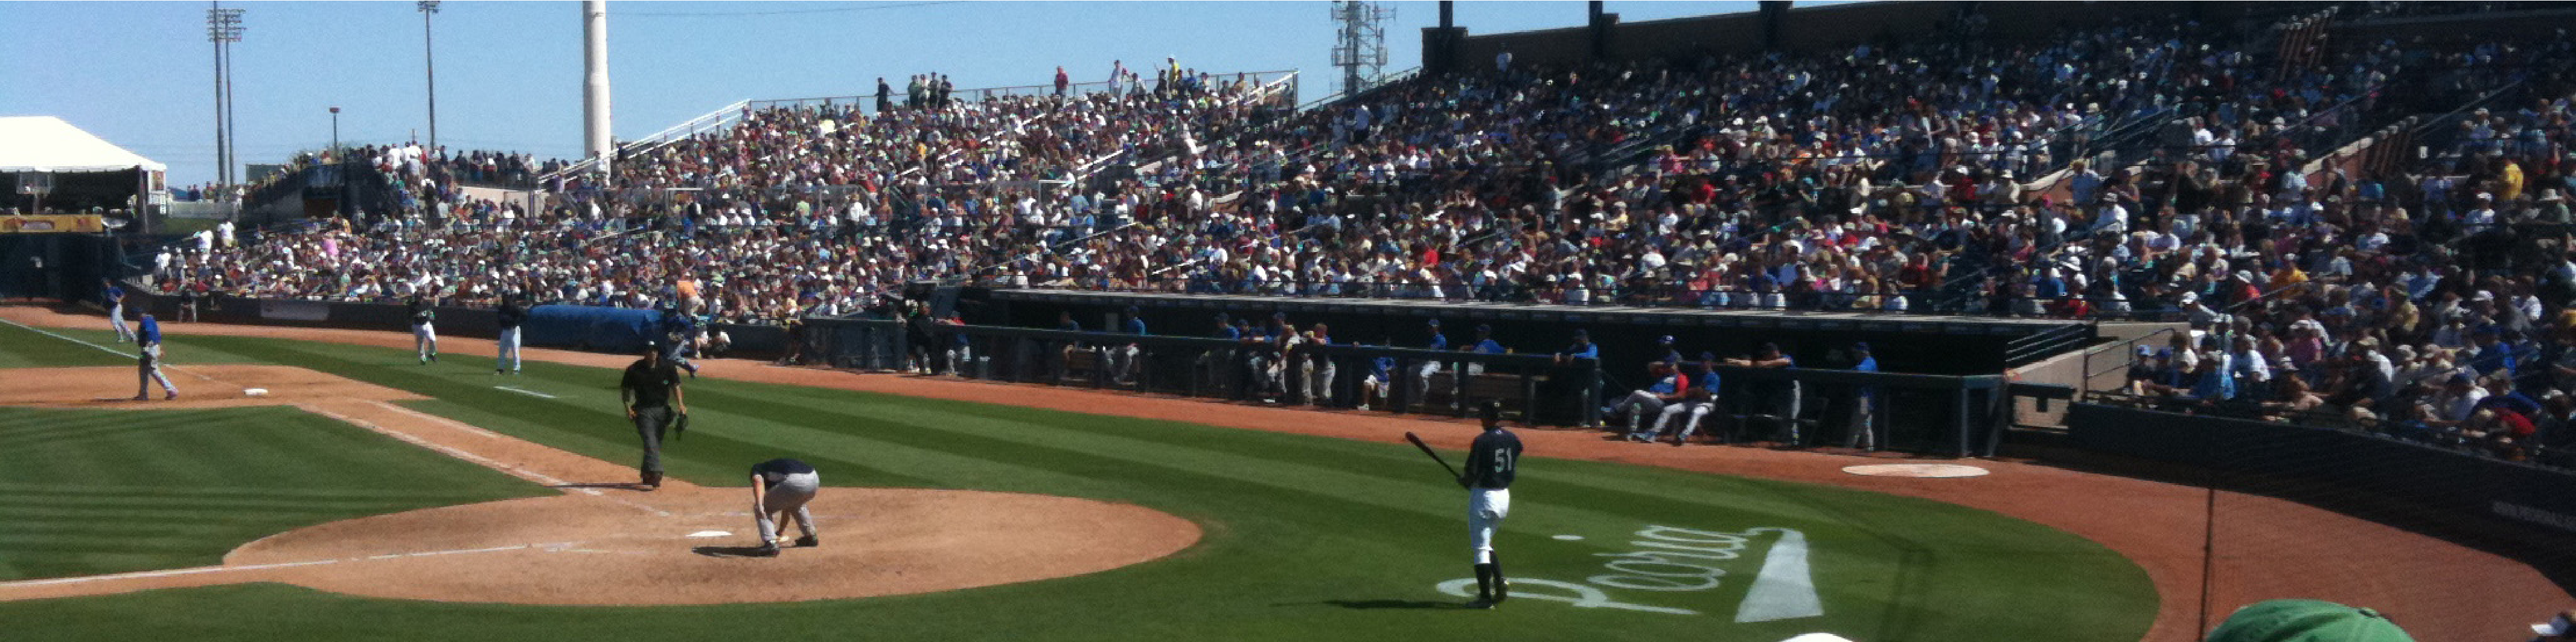
\includegraphics[width=\textwidth]{sampleteaser}
%   \caption{Seattle Mariners at Spring Training, 2010.}
%   \Description{Enjoying the baseball game from the third-base
%   seats. Ichiro Suzuki preparing to bat.}
%   \label{fig:teaser}
% \end{teaserfigure}

% \received{20 February 2007}
% \received[revised]{12 March 2009}
% \received[accepted]{5 June 2009}

%%
%% This command processes the author and affiliation and title
%% information and builds the first part of the formatted document.
\maketitle

\section{Introduction}
\label{sec:intro}

\begin{figure}[!t]
	\centering
	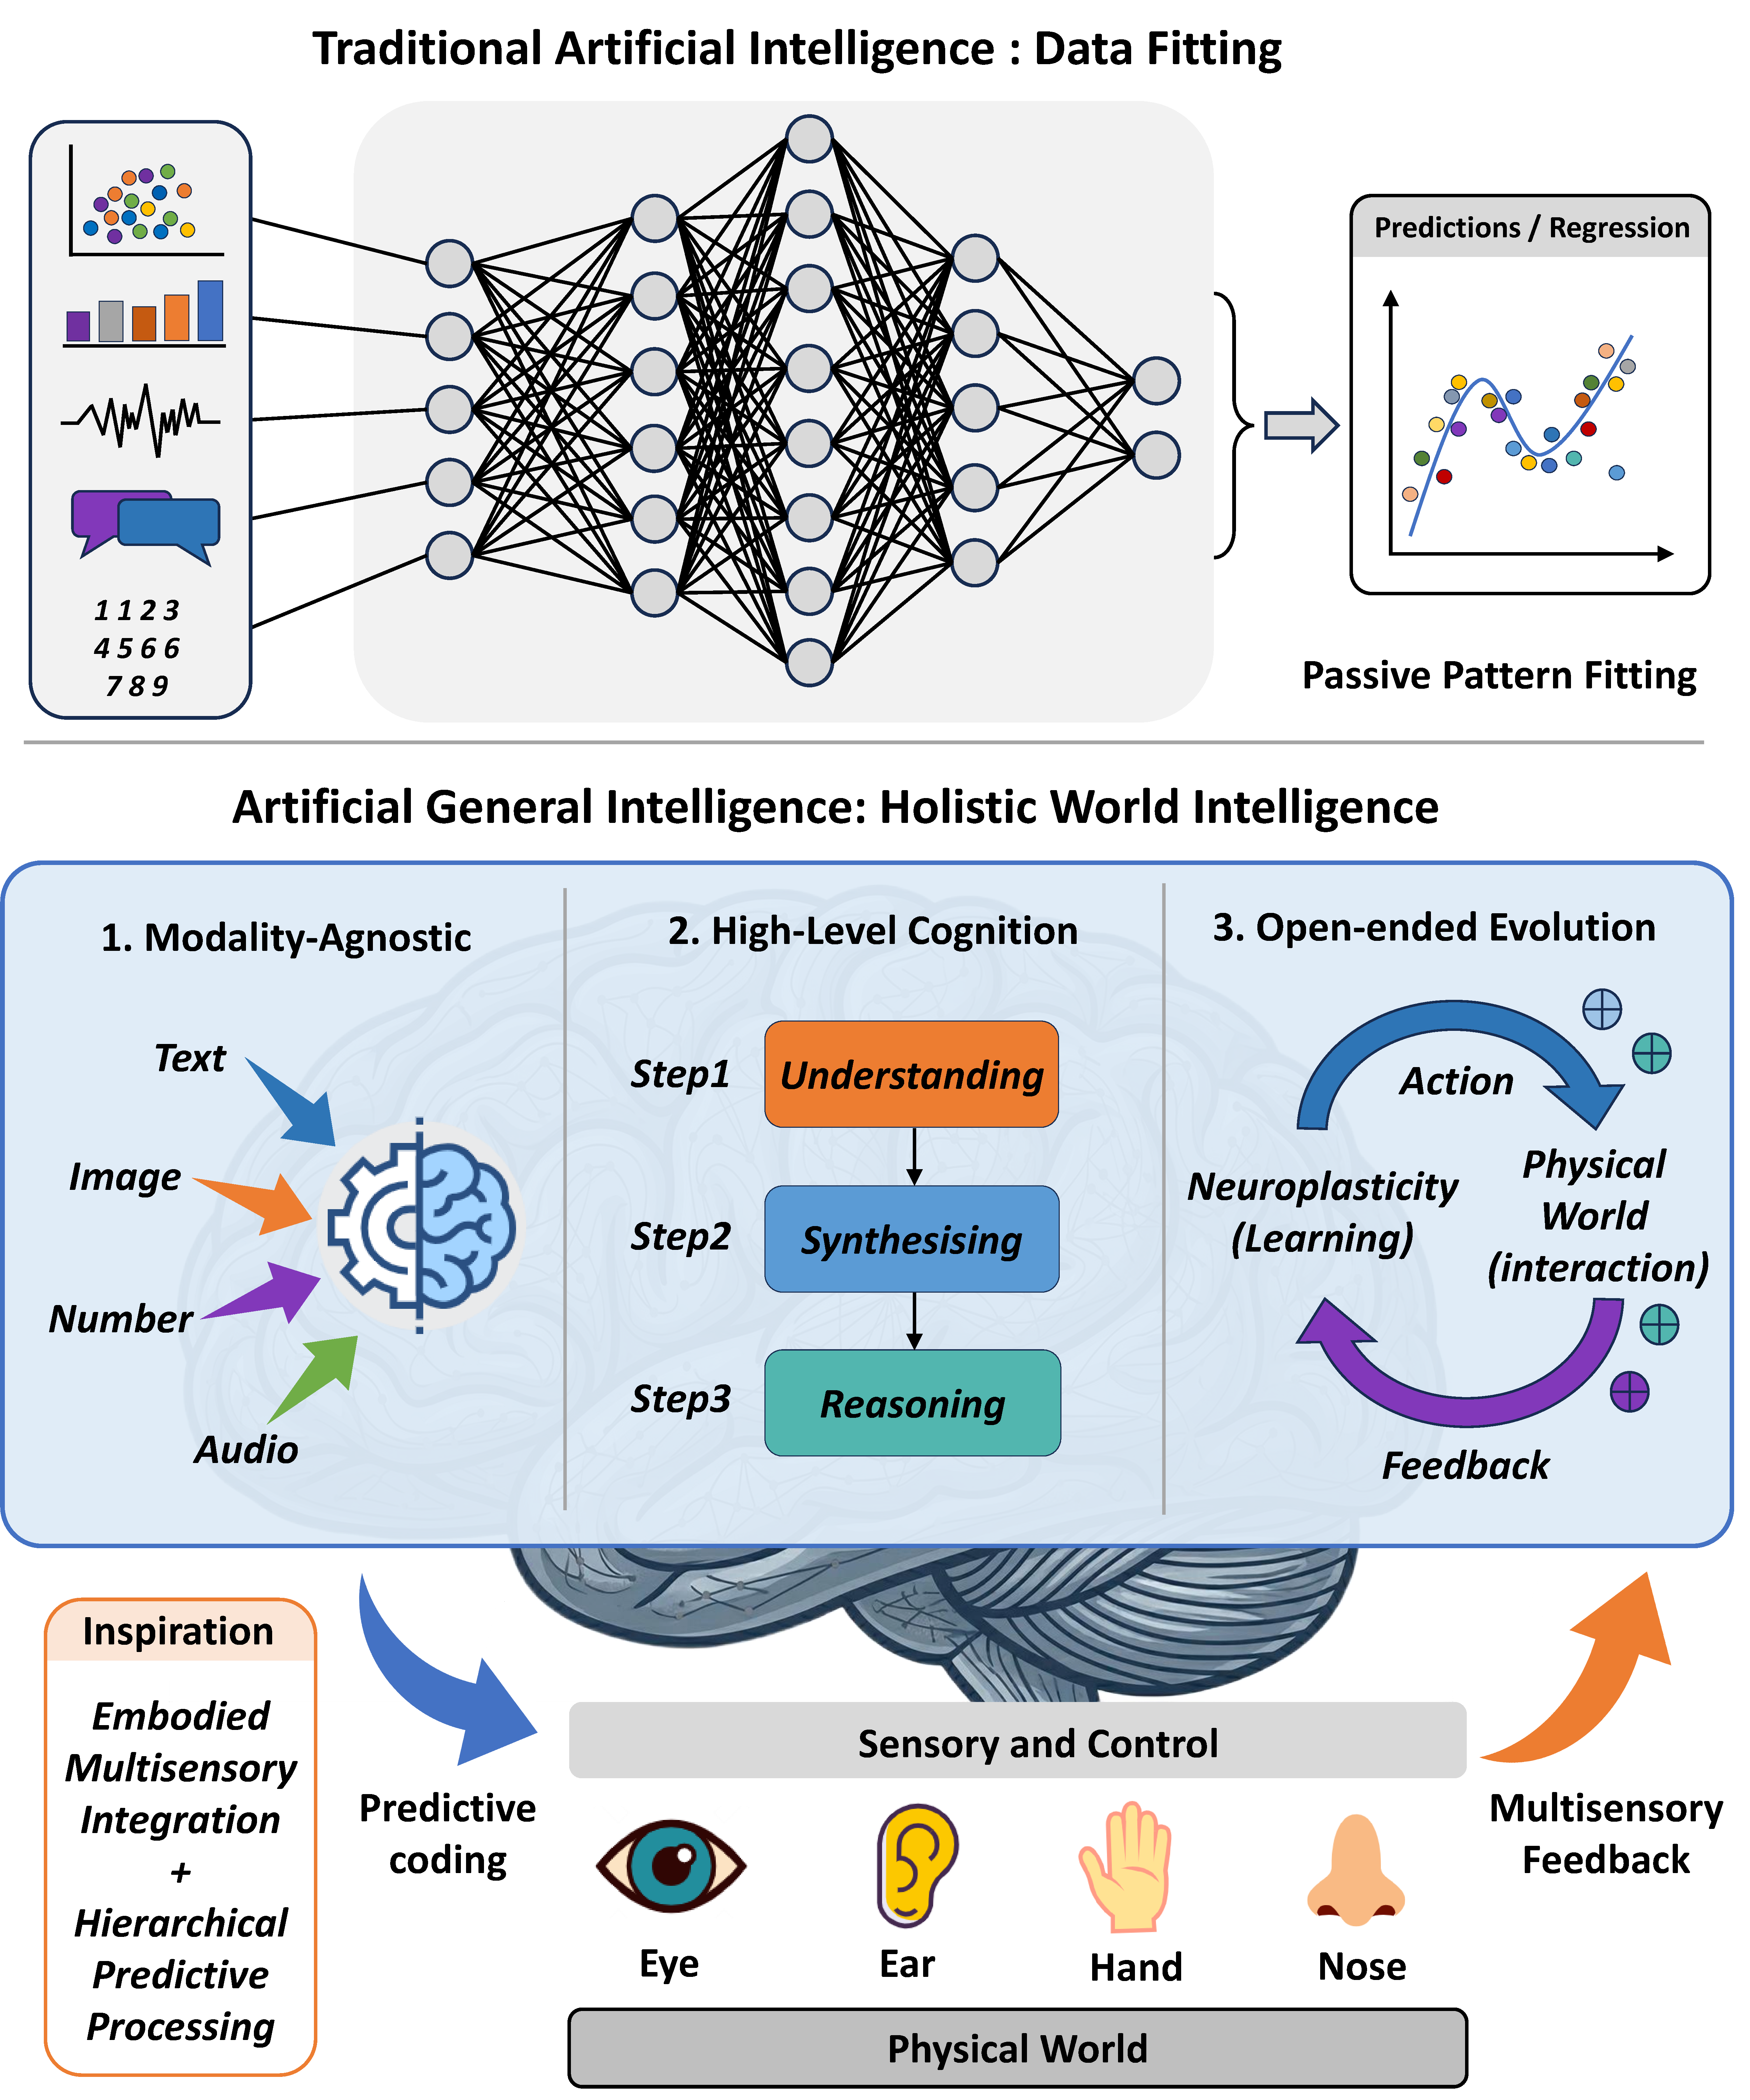
\includegraphics[scale=0.1]{figure/figure22.pdf}
    \vspace{-3mm}
	\caption{The Paradigm Shift from Traditional Statistical Data Fitting to Holistic World Intelligence (HWI) for AGI. }
    \vspace{-5mm}
	\label{figure1}
\end{figure}

\begin{figure*}[!t]
	\centering
	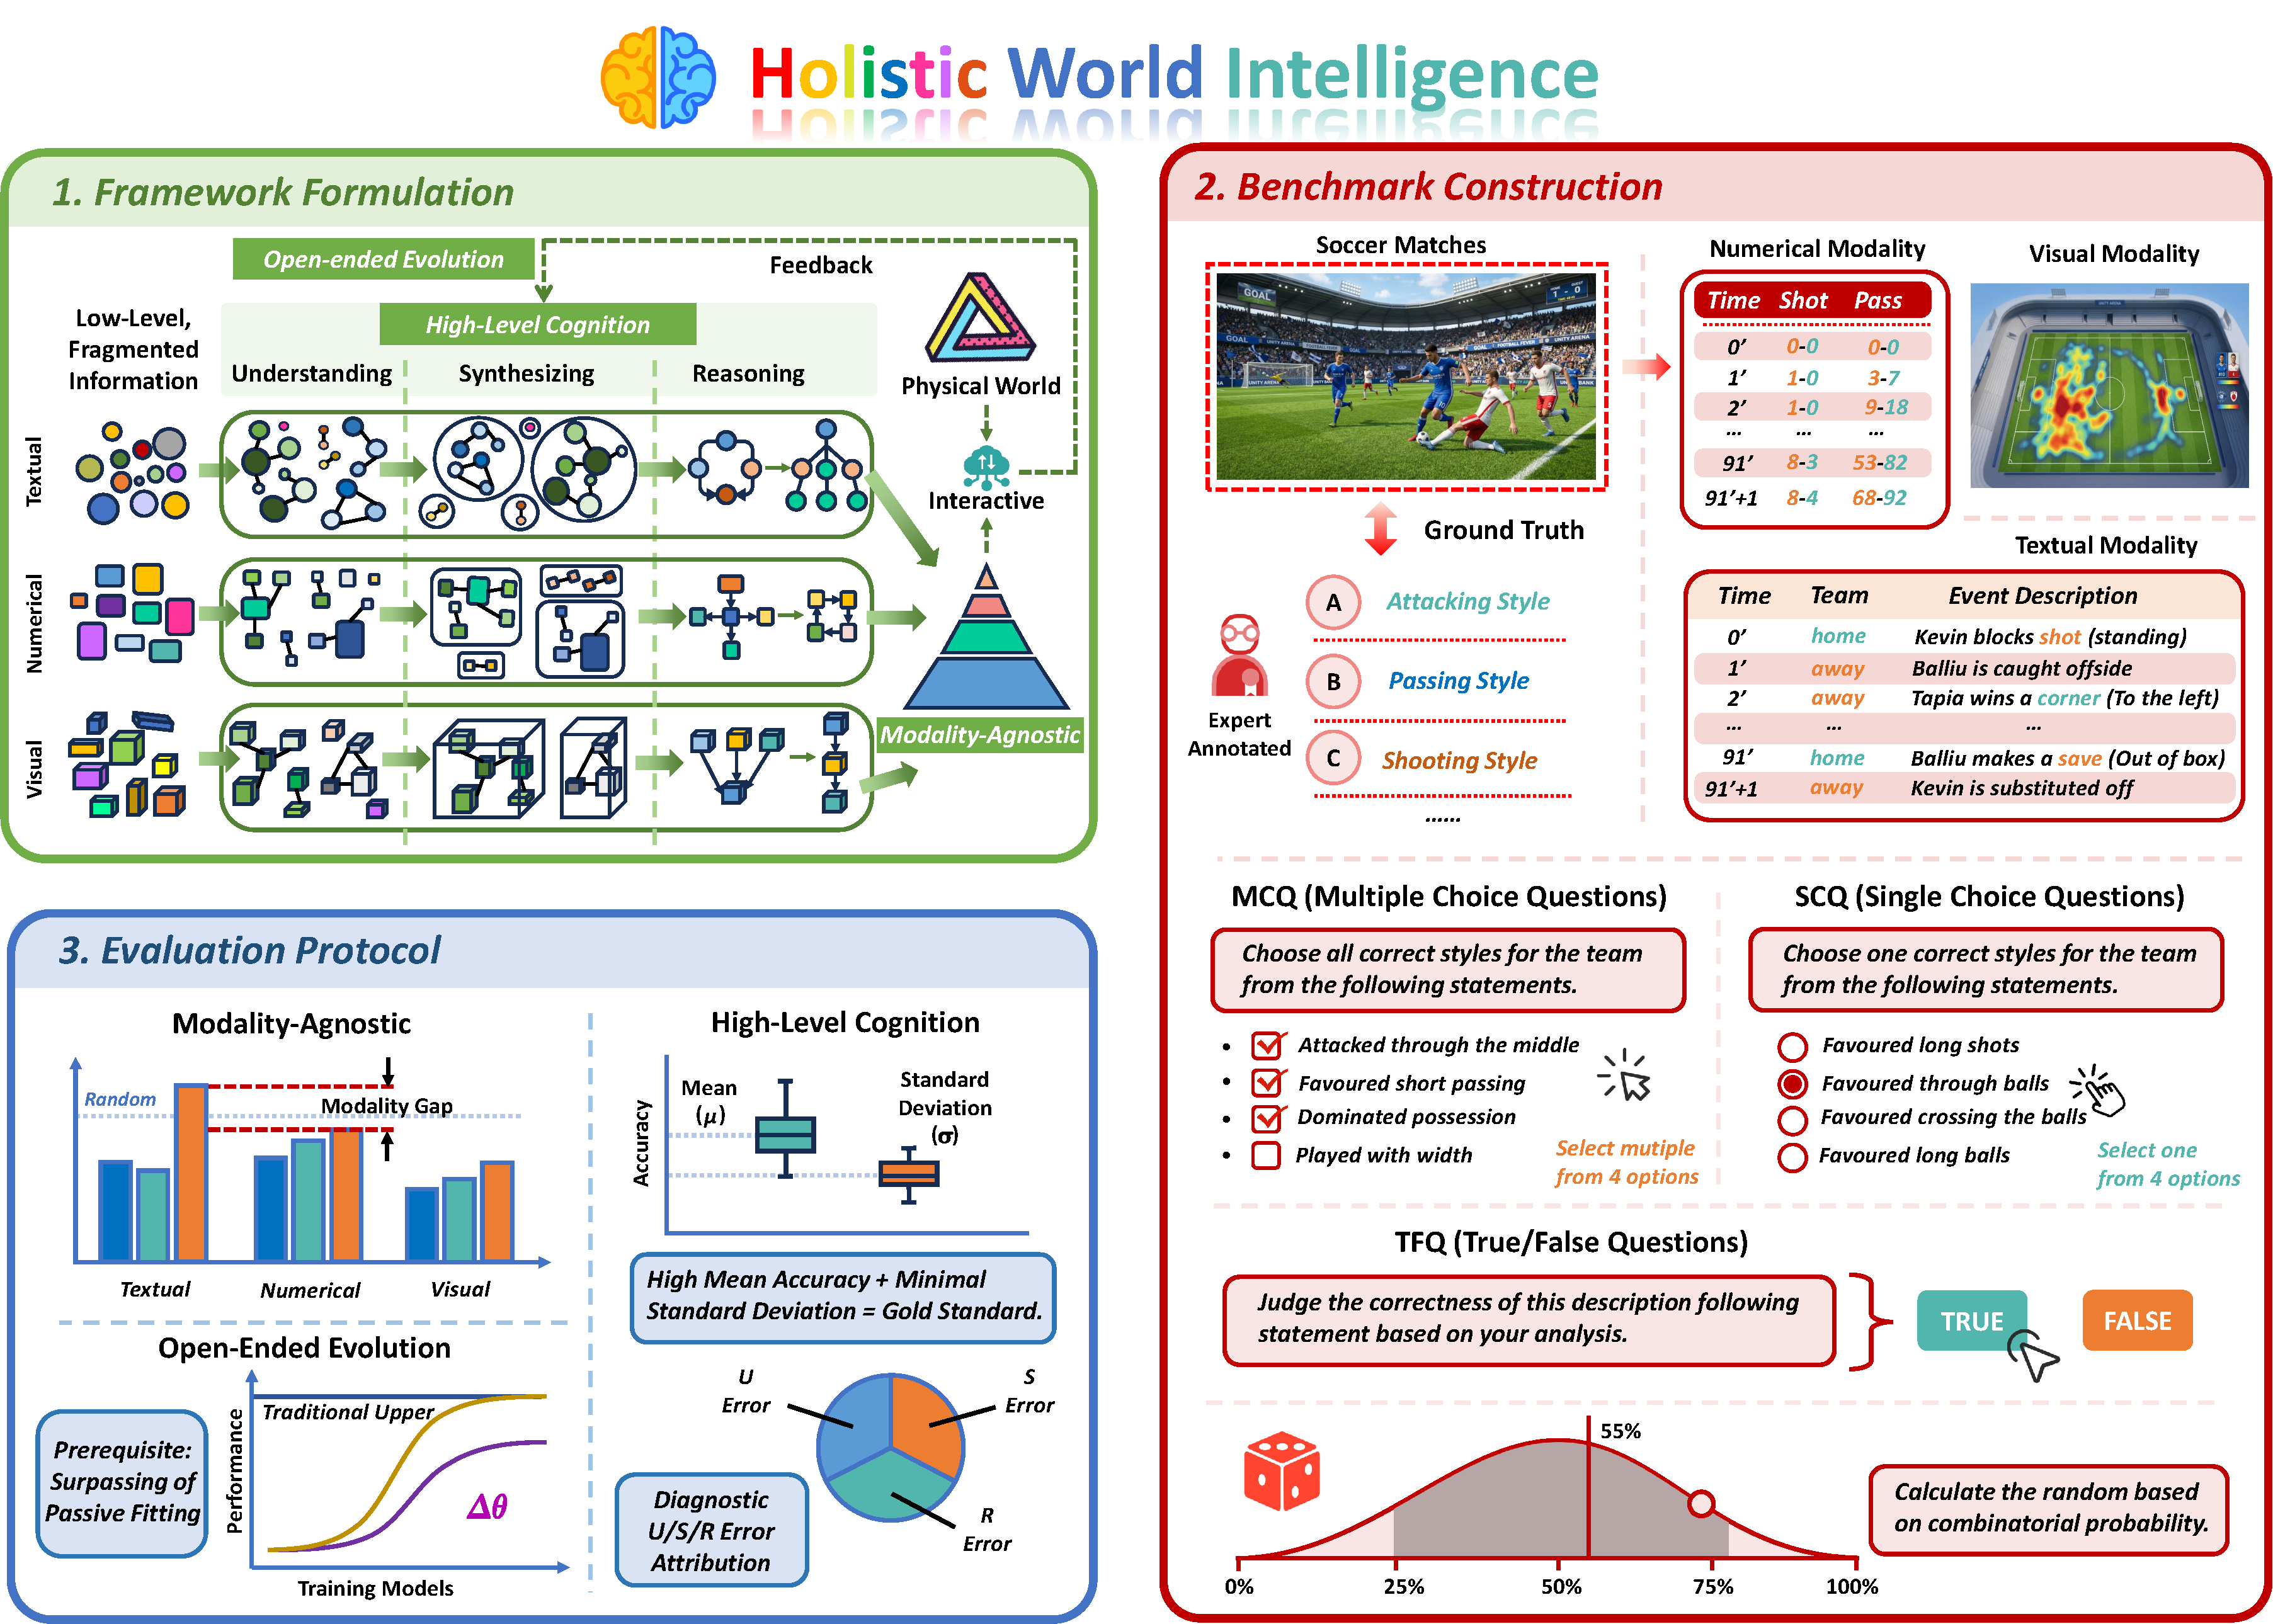
\includegraphics[scale=0.29]{figure/figure2.pdf}
    \vspace{-2mm}
	\caption{The Systematic Paradigm for Evaluating Holistic World Intelligence (HWI) across Multi-modal Representations. }
    \vspace{-3mm}
	\label{figure2}
\end{figure*}

The inherent complexity and heterogeneity of the physical world pose a fundamental bottleneck to the evolution toward Artificial General Intelligence (AGI) \cite{goertzel2014artificial}.
This reality subjects Large Language Models (LLMs), the quintessential paradigm in the pursuit of AGI \cite{bubeck2023paper}, to foundational performance scrutiny \cite{zhao2023survey}.
Profoundly, addressing this bottleneck necessitates a paradigm shift toward \textbf{Holistic World Intelligence} (HWI), an endogenously and perpetually integrated capacity to process heterogeneous real-world representations.
Inspired by cognitive neuroscience represented by Embodied Multisensory Integration \cite{stein2008multisensory} and Hierarchical Predictive Processing \cite{clark2013whatever}, we posit that HWI can be anchored to three core attributes conceptually illustrated in Figure~\ref{figure1}.
First, HWI is inherently \emph{Modality-Agnostic}, enabling the resolution of heterogeneous physical scenarios through unified internal representations that transcend disparate sensory boundaries \cite{ngiam2011multimodal}.
Second, it embodies \emph{High-Level Cognition} (HLC), mimicking the human-like cognitive hierarchy to integrate foundational functions into structured reasoning chains \cite{laird2017standard, bengio2017consciousness}.
Third, it facilitates \emph{Open-ended Evolution}, a neuroplasticity-inspired attribute \cite{hassabis2017neuroscience} that empowers the model to continuously and actively augment its capabilities through autonomous environmental interaction \cite{silver2021reward}.

Despite their prevalence, current approaches fail to internalize these core attributes of HWI.
Predominantly, while attempting to bridge heterogeneity gaps, Multimodal Large Language Models (MLLMs) largely rely on superficial semantic alignment \cite{radford2021learning} rather than achieving a truly Modality-Agnostic unified representation, leaving them fragmented when facing multidimensional physical properties \cite{wu2024next, tong2024eyes}.
Simultaneously, prevailing reasoning paradigms often focus on scaling exogenous logical complexity via externally designed heuristics \cite{wei2022chain, yao2023tree}; however, such plug-and-play enhancements do not translate into genuine endogenous reasoning capabilities or autonomous cognitive depth \cite{huang2023large}.
Most critically, the current framework still remains restricted to modeling the static physical world through passive data-fitting \cite{kaplan2020scaling}, rather than actively exploring and exploiting dynamic environmental feedback to foster sustained, open-ended cognitive growth \cite{wang2023voyager}.
Consequently, these gaps jointly raise a fundamental question: \emph{Can a unified architecture truly internalize the holistic laws of the physical world to attain authentic, world-level intelligence?}

Fundamentally, overcoming these persistent bottlenecks is currently hindered by systemic deficiencies across three critical dimensions.
\emph{Architecturally}, the absence of established HWI-centric datasets and evaluation benchmarks \cite{srivastava2022behavior, gu2023maniskill2} precludes a rigorous and empirical measurement of holistic world representations.
\emph{Theoretically}, a lack of principled analytical guidance consigns the internal mechanisms of world-level cognition to a black box \cite{li2022emergent}, rendering the emergence of HWI largely uninterpretable and opaque \cite{nanda2023progress}.
\emph{Methodologically}, the dearth of novel paradigms capable of triggering endogenous logical growth and continuous environmental interaction prevents a substantive transition from static fitting to active intelligence augmentation \cite{park2023generative}.
To address these multifaceted gaps, this work establishes a structured framework to rigorously analyze the three defining attributes of HWI, providing both theoretical insights and empirical evidence to guide the development of future effective AGI methodologies \cite{bengio2021deep}.

Therefore, this work establishes a holistic and principled evaluation paradigm to bridge the existing gaps between current LLMs and the realization of authentic AGI \cite{mahowald2024dissociating}. Our specific contributions are summarized across three dimensions:
\begin{itemize}[leftmargin=*]
\item \textbf{Systematic Framework and Infrastructure:} We propose a comprehensive framework for \textbf{Holistic World Intelligence}, providing a formal definition of its core attributes (Sec.~\ref{formulation}). To enable empirical measurement, we introduce a specialized benchmark named \textbf{WorldScope} (Sec.~\ref{benchmark}) and a rigorous evaluation protocol (Sec.~\ref{protocol}) to assess the emergence of this capability under heterogeneous real-world representations.
\item \textbf{Empirical Investigation of Capability Collapse:} We conduct an extensive empirical study revealing a critical phenomenon we term \emph{Capability Collapse} in current state-of-the-art multimodal models when processing complex physical data (Sec.~\ref{phenomenon}). By delving into the underlying causes of this failure, we provide a foundational analysis that fills the current void in systematic understanding of world-level performance (Sec.~\ref{analysis}).
\item \textbf{In-depth Analysis and Future Roadmap:} We perform a granular investigation into three pillars of HWI: \emph{Modality-Agnosticism} (Sec.~\ref{modality}), \emph{High-level Cognition} (Sec.~\ref{HLC}), and \emph{Open-ended Evolution} (Sec.~\ref{evolution}). Based on these insights, we propose preliminary improvements and offer a strategic roadmap to guide future efforts toward AGI through LLMs (Sec.~\ref{future}).
\end{itemize}

\begin{table*}[t]
    \centering
    \caption{Comparison of methodologies towards AGI based on the three core attributes of \textbf{Holistic World Intelligence (HWI)}.}
    \vspace{-4mm}
    \label{tab:related_comparison}
    \renewcommand{\arraystretch}{1.0}
    \setlength{\tabcolsep}{4pt} 
    \small 
    \begin{tabularx}{\textwidth}{p{2.8cm} l l X c c c} 
        \toprule
        \textbf{Target Attribute} & \textbf{Major Class} & \textbf{Technical Paradigms} & \textbf{Key Deficiency (vs. HWI)} & \textbf{Mod-A.} & \textbf{HLC} & \textbf{Open-E.} \\
        \midrule
        % 第一组：Modality-Agnostic
        \multirow{2}{*}{\textbf{Modality-Agnostic}} & \multirow{2}{*}{Alignment} 
        & CLIP / Flamingo & Semantically bound to explicit anchors/shortcuts. & \xmark & \xmark & \xmark \\
        & & Knowledge Graphs & Domain-isolated; lacks unified physical grounding. & \xmark & $\triangle$ & \xmark \\
        \midrule
        % 第二组：HLC
        \multirow{2}{*}{\textbf{High-Level Cognition}} & \multirow{2}{*}{Reasoning} 
        & CoT / ToT & Exogenous logic detached from physical constraints. & $\triangle$ & $\triangle$ & \xmark \\
        & & o1 / TTS & Search-based inference without endogenous growth. & $\triangle$ & $\triangle$ & \xmark \\
        \midrule
        % 第三组：Open-E
        \multirow{2}{*}{\textbf{Open-ended Evolution}} & \multirow{2}{*}{Fitting} 
        & Instruction Tuning & Passive interpolation of static, non-interactive data. & $\triangle$ & \xmark & \xmark \\
        & & RLHF / DPO & Reactive optimization lacking proactive world-modeling. & $\triangle$ & $\triangle$ & $\triangle$ \\
        \midrule
        \textbf{All Dimensions} & \textbf{Ours} & \textbf{HWI Framework} & \textbf{Endogenous, grounded, and active intelligence.} & \textbf{\cmark} & \textbf{\cmark} & \textbf{\cmark} \\
        \bottomrule
    \end{tabularx}
    \begin{flushleft}
    \scriptsize
    \textbf{Note}:
    \textbf{Mod-A.}: Modality-Agnostic (transcending sensory boundaries); 
    \textbf{HLC}: High-Level Cognition (endogenously grounded reasoning chains); 
    \textbf{Open-E.}: Open-ended Evolution (active interaction vs. static fitting). 
    \cmark\ indicates strong support; 
    $\triangle$ indicates partial/limited support; 
    \xmark\ indicates little or no support.
    \end{flushleft}
    \vspace{-2mm}
\end{table*}

\begin{table}[t] 
    \centering
    \caption{Summary of existing AGI theoretical perspectives and their gaps relative to the HWI requirements.}
    \vspace{-4mm}
    \label{tab:theory_summary}
    \renewcommand{\arraystretch}{1.0} 
    \setlength{\tabcolsep}{3pt} 
    \footnotesize 
    \begin{tabularx}{\columnwidth}{@{} p{1.3cm} p{2.7cm} X @{}}
        \toprule
        \textbf{Perspective} & \textbf{Core Examples} & \textbf{Primary Gap} \\ 
        \midrule
        \textbf{Optimality} & AIXI, Universal Intelligence & Idealized assumptions; incomputable. \\
        \midrule
        \textbf{Cognitive} & World Models, Active Inference Predictive Processing & Closed environments; modality-specific; limiting unified cross-modal evaluation. \\
        \midrule
        \textbf{Capability} & ARC, Meta-Learning & Static tasks; lacks a unified how-to path. \\
        \midrule
        \textbf{HWI (Ours)} & \textbf{HWI Framework} & \textbf{Integrated, grounded, and evaluable.} \\
        \bottomrule
    \end{tabularx}
    \vspace{-2mm} 
\end{table}

\section{Related Work}
\label{sec:related}

\subsection{Methodological Progress Towards AGI}

Existing AGI methodologies broadly fall into three paradigms (Table~\ref{tab:related_comparison}), each exhibiting systemic deficiencies relative to HWI attributes \cite{marcus2020next}.
First, \textbf{representation alignment} (e.g., contrastive learning, joint embeddings, and models like CLIP \cite{radford2021learning}/Flamingo \cite{alayrac2022flamingo} or Knowledge Graphs \cite{ji2021survey}) maps disparate modalities into shared spaces but remains \emph{semantically bound} to explicit anchors, failing to achieve true \emph{Modality-Agnosticism} \cite{yuksekgonul2022and}.
Second, \textbf{exogenous reasoning} (e.g., CoT, ToT, or search-based paradigms like o1/TTS \cite{snell2024scaling}) facilitates logical transparency yet operates in a reasoning vacuum detached from physical constraints, precluding endogenously grounded \emph{High-Level Cognition} \cite{pearl2018theoretical}.
Finally, \textbf{static optimization} via instruction tuning or preference learning (RLHF \cite{ouyang2022training}, DPO \cite{rafailov2023direct}) approximates world states through passive data-fitting \cite{bender2020climbing}. Lacking active environmental interaction, these methods cannot sustain \emph{Open-ended Evolution} \cite{lehman2011abandoning}.
The HWI framework is therefore explicitly designed to evaluate and bridge these fundamental gaps between current paradigms and authentic world intelligence \cite{bisk2020experience}.

\vspace{-2mm}
\subsection{Theoretical Progress Towards AGI}

Theoretical studies of AGI have formalized \emph{intelligence} from several distinct but incomplete perspectives (Table~\ref{tab:theory_summary}) \cite{legg2007collection}.
First, \textbf{optimality-based theories} (e.g., AIXI \cite{hutter2005universal}, Universal Intelligence \cite{legg2007universal}) define generality through asymptotic performance across environments \cite{sutton1998reinforcement}.
While principled, they rely on idealized and often incomputable assumptions \cite{leike2017ai}, remaining descriptive rather than executable for real-world interactive intelligence \cite{everitt2018agi}.
Second, \textbf{cognitive and world-model theories} (e.g., World Models \cite{ha2018recurrent}, Predictive Processing \cite{friston2010free}, Active Inference \cite{zhiren2026learning}) emphasize endogenous modeling, prediction, and action \cite{matsuo2022deep}.
Although closer to authentic intelligence, they are typically grounded in specific modalities or closed environments \cite{kaiser2019model}, limiting unified cross-modal evaluation under open-world complexity \cite{hafner2019dream}.
Third, \textbf{capability-oriented theories} (e.g., ARC \cite{chollet2019measure}, meta-learning \cite{finn2017model}) characterize AGI through abstraction, reasoning, and rapid generalization \cite{lake2017building}.
However, they mainly specify \emph{what} capabilities to test, rather than \emph{how} to construct a unified intelligence framework \cite{lecun2022path}, and their largely static tasks are insufficient for continuous interaction and open-ended evolution \cite{team2021open}.
Overall, existing AGI theories clarify important aspects of intelligence, but still lack a unified path from abstract formulation to systematic real-world evaluation \cite{bommasani2021opportunities}.
Our HWI framework addresses this gap through an integrated structure spanning \textbf{framework}, \textbf{benchmark}, and \textbf{protocol}.

\section{Holistic World Intelligence} 
\label{sec:mhlc-benchmark}
\subsection{Framework}
\label{formulation}
Based on the three core attributes of Holistic World Intelligence capabilities in Figure ~\ref{figure2}, we formalize its definition as follows:

1) \textbf{Modality-Agnostic}. Confronted with the complex and heterogeneous representations of the physical world, HWI relies on an underlying, ubiquitous processing mechanism. 
For any given modality $m \in \{\text{num}, \text{vis}, \text{text}, \dots\}$, the macroscopic so-called holistic mechanism of HWI, denoted as $\mathcal{F}$, must satisfy the representational equivalence \cite{baltruvsaitis2018multimodal}. 
Specifically, when disparate modalities $m_a$ and $m_b$ observe the same objective physical event $\mathcal{E}$, this mechanism must transcend representational barriers to ensure absolute consistency in the derived conclusions, fundamentally eliminating reliance on modality-specific or explicit semantic shortcuts:
\begin{equation}
\label{eq1}
\mathcal{F}(\mathcal{X}^{m_a}) \equiv \mathcal{F}(\mathcal{X}^{m_b}) \rightarrow \mathbf{y}_{\mathcal{E}}.
\end{equation}

2) \textbf{High-Level Cognition}. The essence of processing the complex physical world lies in bridging the representational chasm between low-level data and high-dimensional principles. Furthermore, High-Level Cognition can be defined as the transitional process of deriving high-level conclusions from low-level and fragmented foundational information, which can be instantiated as an \emph{Understanding-Synthesizing-Reasoning chain} structure ($f_R \circ f_S \circ f_U$) \cite{liu2025can}. We introduce this paradigm to process heterogeneous physical observations $\mathcal{X}^{m}$: 
\begin{itemize}[leftmargin=*]
    \item \textbf{Understanding-U} ($f_U$): Operates independently on each fragmented, low-level physical segment to extract isolated local features: $\mathcal{H}_{local}^{m} = \{ f_{U}(x_{i}^{m}) \}_{i=1}^{N_{m}}$. 
    \item \textbf{Synthesizing-S} ($f_S$): Integrates all fragmented local features to construct a coherent global representation: $\mathbf{H}_{global}^{m} = f_{S}(\mathcal{H}_{local}^{m})$.
    \item \textbf{Reasoning-R} ($f_R$): Derives high-level conclusions regarding the physical world (e.g., high-dimensional intentions, macroscopic laws) based on this global representation: $\mathbf{y} = f_{R}(\mathbf{H}_{global}^{m})$.
\end{itemize}

3) \textbf{Open-ended Evolution}. Analogous to neuroplasticity in the human brain, the model must achieve continuous reshaping of its endogenous logic through dynamic interaction with the physical environment \cite{parisi2019continual}. This dynamic process exhibits an iterative, upward trajectory alongside the interaction step $t$:
\begin{equation}
\label{eq2}
\theta^{(t+1)} = \theta^{(t)} + \Delta \theta \left( \mathcal{X}_{t}^{m}, \text{Feedback}_{t}, \mathcal{F}_{\theta^{(t)}} \right).
\end{equation}
This ensures the model can continuously shatter its inherent cognitive boundaries and seamlessly adapt to the open-ended, boundless, and complex evolution of the physical world.

\begin{figure}[!t]
	\centering
	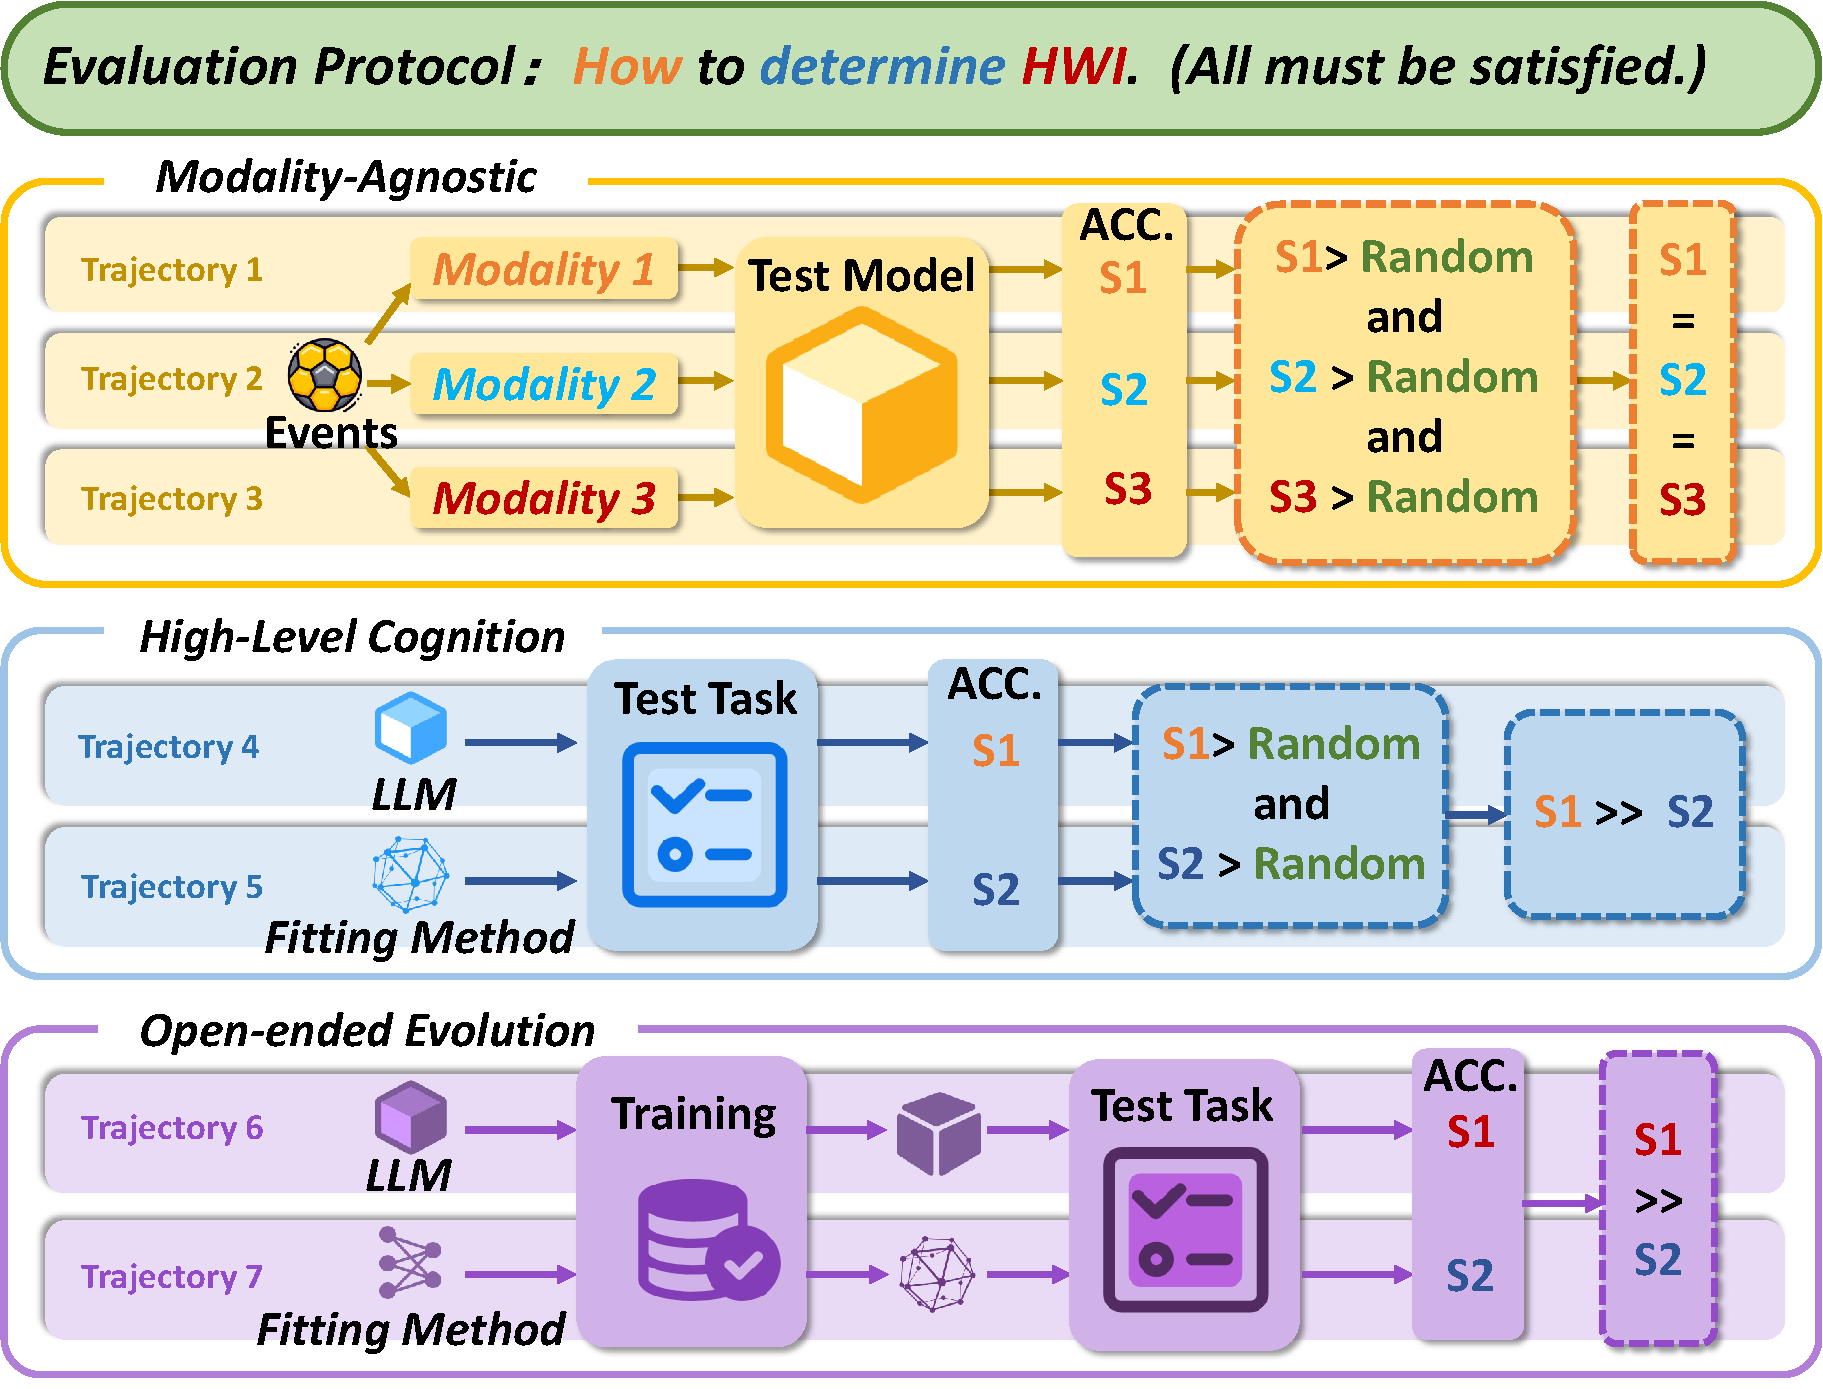
\includegraphics[scale=0.27]{figure/figure21.pdf}
    \vspace{-3mm}
	\caption{Evaluation and Diagnosis pipeline (How to test three capabilities under HWI framework). }
    \vspace{-3mm}
	\label{figure...}
\end{figure}

\subsection{WorldScope Benchmark}
\label{benchmark}

Existing benchmarks predominantly evaluate superficial perception, failing to test models' capacity to \emph{transcend low-level representational barriers} and \emph{formulate high-order macroscopic conclusions}. To address this gap, we introduce \textbf{WorldScope}, a dedicated benchmark for evaluating Holistic World Intelligence, constructing on professional football matches from WhoScored. With the aim at complex physical world characterized by high-dimensional adversarial dynamics, this testbed can rigorously assesses models' HWI capacity boundary. Concretely, WorldScope consists of \emph{two strictly decoupled components} with details in Appendix~\ref{app:construction_pipeline}:
\begin{itemize}[leftmargin=*]
\item \textbf{Low-level Multimodal Input:} We extract fine-grained, fragmented observations for each match, including discrete numerical statistics (e.g., passes, zones), chronological textual commentary, and visual positional heatmaps of all players, while depicting the underlying physical world.
\item \textbf{High-level Integrated Output:} Macroscopic team-style summaries are extracted from various Expert Match Reports and normalized into a finite set of 12 tactical playing styles, which cannot be trivially deduced from isolated foundational data.
\end{itemize}

These strictly decoupled components then perfectly operationalizes our theoretical framework. 
(1) First, by capturing the exact same objective physical event across three heterogeneous channels, the benchmark inherently demands \textbf{Modality-Agnostic} processing, preventing models from exploiting modality-specific semantic shortcuts. 
(2) Furthermore, bridging the representational chasm between raw, fragmented signals and macroscopic tactical labels necessitates genuine \textbf{High-Level Cognition}. Specifically, a model must first perform \textit{understanding} by extracting isolated local features from fragmented inputs (e.g., recognizing discrete passes or shots event from numerical counts, textual commentary, or visual density spots). Next, it must execute \textit{synthesizing} by integrating these scattered events into a coherent global representation (e.g., a panoramic view of the overall match dynamics). Finally, through \textit{reasoning}, it maps this unified representation to high-level conclusions (e.g., deducing macroscopic tactical styles like "favoured short passing"). This process comprehensively forces the model to execute a complete "Understanding-Synthesizing-Reasoning" (U/S/R) cognitive chain. 
(3) Crucially, our continuous real-world football seasons inherently supports \textbf{Open-ended Evolution}. This provides an infinitely renewable environment, allowing models to not only be statically evaluated but also continuously trained to adapt to novel tactical trends, thereby iteratively evolving their alignment with real-world dynamics. 

% Because new matches and expert reports are generated perpetually, the dataset seamlessly scales without the bottleneck of expensive human annotation.
% We curated a substantial dataset of 5,000 matches to ensure robust evaluation. 

As for benchmark's diversity and richness, to mitigate the ambiguity of HWI evaluation, we formulate the testbed into standardized objective tasks: Multiple Choice Questions (MCQ), Single Choice Questions (SCQ), and True/False Questions (TFQ). For consistency, instruction semantics are strictly aligned across all modalities. We also adopt Exact-Match (EM) as accuracy metric after filtering, where any generated content falling outside the finite acceptable ground truth set is categorically penalized as an incorrect response during HWI evaluation.


\begin{table*}[t]
    \centering
    \caption{Comprehensive performance comparison on three modalities (textual, numerical, and visual) and three tasks (MCQ, SCQ, and TFQ). $\dagger$ denotes theoretically calculated values. }
    \vspace{-2mm}
    \label{tab:main_results_hierarchical}
    \renewcommand{\arraystretch}{1.0} 
    \setlength{\tabcolsep}{14pt} % 
    \begin{tabular}{@{} l l c c c c @{}}
        \toprule
        \multirow{2}{*}{\textbf{Category}} & \multirow{2}{*}{\textbf{Model}} & \multirow{2}{*}{\textbf{Params}} & \multicolumn{3}{c}{\textbf{Accuracy (\%)}} \\
        \cmidrule(lr){4-6} 
        & & & \textbf{MCQ} & \textbf{SCQ} & \textbf{TFQ} \\
        \midrule
        
        % ==========================================
        % 基线部分
        % ==========================================
        Baseline & Random-Level & - & 12.95$^\dagger$ & 30.81$^\dagger$ & 56.74$^\dagger$ \\
        \midrule
        
        % ==========================================
        % 文本模态
        % ==========================================
        \rowcolor{blue!10} \multicolumn{6}{c}{\textit{Textual Modality}} \\
        \midrule

        \multirow{6}{*}{General (Zero-Shot)} 
         &  GPT-5.4 \cite{singh2025openai} & - & $\underline{15.00} \pm 3.16$ & $\underline{36.20} \pm 4.87$ & $\underline{54.23} \pm 5.11$ \\
        & Claude-4.6-opus \cite{mukherjee2026red} & - & $14.40 \pm 2.06$ & $33.20 \pm 4.53$ & $53.54 \pm 2.28$ \\
        & Llama-3.1 \cite{grattafiori2024llama} & ~70B & $11.60 \pm 3.26$ & $35.60 \pm 6.62$ & $53.47 \pm 6.30$  \\
        & Mistral-Small-3 \cite{liu2026ministral} & ~24B & $9.00 \pm 4.20$ & $33.60 \pm 5.95$ & $50.89 \pm 3.81$ \\
        & Qwen-2.5 \cite{yang2025qwen3} & ~3B & $\textcolor{blue}{7.20} \pm 2.71$ & $20.80 \pm 5.11$ & $\textcolor{blue}{38.13} \pm 6.72$ \\
        & vicuna-1.5 \cite{zheng2023judging} & ~7B & $8.40 \pm 1.36$ & $\textcolor{blue}{14.60} \pm 1.62$ & $50.00 \pm 0.00$ \\
        \cmidrule(l){2-6} 
        
        \multirow{3}{*}{Traditional Architecture} 
        & \textbf{LSTM} \cite{hochreiter1997long} & ~4.60M &  $20.00 \pm 3.85$ & $\mathbf{\textcolor{red!60!black}{37.20}} \pm 4.07$ & $\mathbf{\textcolor{red!60!black}{61.74}} \pm 2.27$ \\
        & \textbf{MLP} \cite{rumelhart1986learning} & ~3.98M & $17.20 \pm 1.47$ & $ 33.60 \pm 2.24$ & $58.28 \pm 2.77$ \\
        & \textbf{GRU} \cite{cho2014learning} & ~4.44M & $\mathbf{\textcolor{red!60!black}{21.00}} \pm 2.28$ & $ 36.60 \pm 3.79$ & $60.05 \pm 2.26$ \\
        \midrule

        % ==========================================
        % 数字模态
        % ==========================================
        \rowcolor{orange!10} \multicolumn{6}{c}{\textit{Numerical Modality}} \\
        \midrule
        
        \multirow{6}{*}{General (Zero-Shot)} 
        &  GPT-5.4 \cite{singh2025openai} & - & $10.40 \pm 2.94$ & $33.40 \pm 6.89$ & $54.22 \pm 6.22$ \\
        & Claude-4.6-opus \cite{mukherjee2026red} & - & $\underline{14.40} \pm 3.61$ & $\underline{36.40} \pm 8.27$ & $\underline{56.36} \pm 8.92$  \\
        & Llama-3.1 \cite{grattafiori2024llama} & ~70B & $6.40 \pm 2.42$ & $25.40 \pm 5.54$ & $54.21 \pm 8.67$ \\
        & Mistral-Small-3 \cite{liu2026ministral} & ~24B & $\textcolor{blue}{5.80} \pm 2.64$ & $22.40 \pm 4.88$ & $53.03 \pm 4.53$ \\
        & Qwen-2.5 \cite{yang2025qwen3} & ~3B & $6.00 \pm 0.63$ & $24.80 \pm 3.37$ & $\textcolor{blue}{36.84} \pm 5.95$ \\
        & vicuna-1.5 \cite{zheng2023judging} & ~7B & $12.40 \pm 1.74$ & $\textcolor{blue}{13.80} \pm 0.98$ & $50.00 \pm 0.00$ \\
        \cmidrule(l){2-6} 
        
        \multirow{3}{*}{Traditional Architecture} 
        & \textbf{CNN} \cite{lecun1989backpropagation} & ~0.40M & $23.80 \pm 3.31$ & $ 36.80 \pm 4.71$ & $63.38 \pm 5.65$ \\
        & \textbf{MLP} \cite{rumelhart1986learning} & ~0.43M & $\mathbf{\textcolor{red!60!black}{28.40}} \pm 4.22$ & $\mathbf{\textcolor{red!60!black}{38.80}} \pm 6.68$ & $\mathbf{\textcolor{red!60!black}{63.87}} \pm 4.37$ \\
        & \textbf{GRU} \cite{cho2014learning} & ~0.25M & $24.00 \pm 4.82$ & $32.40 \pm 5.78$ & $60.48 \pm 3.48$ \\
        \midrule
        
        % ==========================================
        % 图像模态
        % ==========================================
        \rowcolor{green!10} \multicolumn{6}{c}{\textit{Visual Modality}} \\
        \midrule
        
        \multirow{6}{*}{General (Zero-Shot)} 
        &  GPT-5.4 \cite{singh2025openai} & - & $8.60 \pm 0.49$ & $26.80 \pm 2.56$ & $52.02 \pm 2.39$ \\
        & Claude-4.6-opus \cite{mukherjee2026red} & - & $11.40 \pm 1.36$ & $\underline{30.60} \pm 5.00$ & $\underline{56.59} \pm 3.55$ \\
        &  Llama-3.2-Vision \cite{grattafiori2024llama} & ~90B &  $7.60 \pm 1.36$ & $21.00 \pm 2.28$ & $\textcolor{blue}{32.55} \pm 4.28$  \\
        & Mistral-Small-3.1 \cite{liu2026ministral} & ~24B & $9.00 \pm 3.63$ & $30.20 \pm 4.26$ & $55.00 \pm 1.89$ \\
        & Qwen-2.5-VL \cite{bai2025qwen3} & ~3B & $\underline{12.00} \pm 2.19$ & $14.80 \pm 3.76$ & $49.26 \pm 5.52$ \\
        & LLaVa-1.5 \cite{liu2024improved} & ~7B & $\textcolor{blue}{5.40} \pm 0.49$ & $\textcolor{blue}{13.40} \pm 2.58$ & $50.00 \pm 0.00$  \\
        \cmidrule(l){2-6}
        
        \multirow{3}{*}{Traditional Architecture} 
        & \textbf{ResNet-18} \cite{he2016deep} & ~11.31M & $21.40 \pm 2.58$ & $35.00 \pm 5.40$ & $62.26 \pm 5.33$ \\
        & \textbf{DenseNet-121} \cite{huang2017densely} & ~7.22M & $23.20 \pm 2.79$ & $35.20 \pm 4.71$ & $60.47 \pm 2.26$ \\
        & \textbf{EfficientNet-B0} \cite{tan2019efficientnet} & ~4.34M & $\mathbf{\textcolor{red!60!black}{24.40}} \pm 2.94$ & $\mathbf{\textcolor{red!60!black}{37.60}} \pm 4.72$ & $\mathbf{\textcolor{red!60!black}{63.11}} \pm 1.85$ \\
        
        \bottomrule
    \end{tabular}
    \vspace{-2mm}
\end{table*}



\subsection{Evaluation Protocol}
\label{protocol}

To systematically bridge the empirical results through WorldScope Benchmark with the theoretical foundations under HWI framework, we establish a rigorous evaluation protocol to shift the theoretical perspective to a verifiable sanity check. In this view, the protocol is specifically designed to diagnose quantitatively whether the tested model sufficiently exhibits three formalized attributes of HWI.

1) \textbf{Modality-Agnostic Check:} \emph{Cross-Modality Alignment.} 
To empirically validate the representational equivalence ~\ref{eq1}, we evaluate models independently across numerical ($m_{num}$), textual ($m_{text}$), and visual ($m_{vis}$) modalities for the same split of objective physical events $E$. 
% A model possessing true HWI should yield highly consistent predictive results regardless of the input modality. 
By juxtaposing the performance across heterogeneous input channels, we can measure this modality gap. 
% Crucially, this evaluation must be strictly anchored against a mathematical random baseline. 
% Comparing against random chance is theoretically imperative to establish foundational validity; mere consistency across modalities is mathematically meaningless if the model is systematically hallucinating or guessing. 
% However, exceeding the random baseline is merely a necessary prerequisite, not a sufficient condition. 
To truly prove models' holistic mechanism $\mathcal{F}$ transcending representational barriers, a model must simultaneously satisfy two rigorous criteria: (1) it must significantly exceed the \emph{random baseline} across all modalities, and (2) it must exhibit a \emph{minimized modality gap}.
% Macro-statistical convergence is deceptive if a model correctly predicts disjoint subsets of samples across different modalities. 
In this case, genuine Modality-Agnosticism mandates that for any specific physical event $E_i \in E$, the derived macroscopic truth $y_i$ must remain invariant across $m_{num}$, $m_{text}$, and $m_{vis}$. 
Then, by sanity check on degradation among modalities, a persistent reliance on modality-specific semantic shortcuts is exposed, thereby invalidating any claim of modality-agnostic capability.


2) \textbf{High-Level Cognition Check:} \emph{Statistical Aggregation and Diagnostic Attribution for $f_R \circ f_S \circ f_U$.} 
To quantify a model's capacity to execute the "Understanding-Synthesizing-Reasoning" chain, we introduce a mean-and-standard-deviation ($\mu \pm \sigma$) profiling strategy. 
First, we need to check \emph{whether models are capable of HLC capability}.
In this case, we have mean accuracy $\mu$ serving as the primary indicator of model's absolute capacity to successfully complete the full mapping from fragmented inputs to high-order conclusions as $y = f_R(f_S(f_U(x)))$, while the standard deviation $\sigma$ quantifies the internal stability of this cognitive chain against data variance. 
Here, models are required to surpass the boundary achieved by task-specific traditional-architecture models with passive data-fitting to empirically establish the genuine, intrinsic emergence of HLC.
Futhermore, we need to check \emph{whether models have the intrinsic ability of HLC capability}.
% Because these compact architectures establish a physical upper bound for "passive data-fitting" within a closed data distribution, a massive foundation model that fails to outperform them in a zero-shot setting fundamentally demonstrates an inability to autonomously construct a genuine endogenous reasoning chain.
% If a model's pre-trained, generalized cognitive capacity is inferior to simple statistical interpolation, any claim of possessing High-Level Cognition is entirely invalidated.  
To pinpoint exact structural bottlenecks when this cognition fails, we introduce a diagnostic U/S/R error attribution mechanism in Appendix ~\ref{sec:usrules}). 
This allows us to deconstruct incorrect predictions and identify precisely which specific sub-function—local feature extraction $f_U$, global integration $f_S$, or high-dimensional deduction $f_R$—fractures when processing complex physical signals.

3) \textbf{Open-ended Evolution Check:} \emph{Evolutionary Baselines vs. Superficial Fitting.} 
Our formulation \ref{eq2} mandates that an intelligent agent can autonomously and structurally reshape its internal logic through environmental interaction. 
To investigate this potential, we benchmark general LLMs against two distinct reference points: traditional task-specific supervised models and fully fine-tuned LLMs. 
Here, traditional-architecture models establish a physical upper bound for "passive data-fitting". 
By further evaluating LLMs before and after task-specific fine-tuning, we can diagnose the nature of their learning and evolution capabilities. 
If the fine-tuned LLMs still fail to surpass the traditional-architecture baselines, it constitutes powerful \emph{counter-evidence} indicating that the parameter updates merely resulted in superficial overfitting to task distribution, rather than triggering the genuine, endogenous structural cognitive growth required for true open-ended evolution.
\vspace{-2mm}

\section{Experiment}
\label{sec:experiment}
\subsection{Experimental Setup}
\textbf{Dataset Configurations}. The experiments are performed on WorldScope benchmark comprising 5,000 examples in total, with 4,500 examples for training and 500 for testing. All models will be tested on the same test split with \emph{three assessment forms} (SCQ, MCQ, and TFQ), and instantiated via prompt templates for \emph{three modality inputs} (textual, numerical, and visual).

\textbf{Comparison Models}. To provide sufficient experimental evidence for subsequent argumentation under protocal in ~\ref{protocol}, we will test with SOTA LLMs of various modalities on the same backbone families before and after fine-tuning, while taking traditional architecture models as the capability boundary of passive data-fitting method. The full experiment details including model list, input formatting, training, and hyperparameters) are given in Appendix ~\ref{sec:training-protocol}.


\subsection{Main Result and Analysis}
\label{phenomenon}

Table ~\ref{tab:main_results_hierarchical} presents a comprehensive performance comparison across textual, numerical, and visual modalities, encompassing general-purpose LLMs alongside the capability boundary of the passive data-fitting method presented by task-specific traditional-architecture models. The empirical data intuitively reveals several highly counter-intuitive phenomena exhibited by these SOTA LLMs confronting complex physical world representations.

1) \textbf{The Inverse Scaling Phenomenon.}
Contemporary AI development relies heavily on \emph{Scaling Laws}, which posit that model capabilities scale monotonically with parameter count. 
However, our experimental results reveal a counter-intuitive "inverse scaling" phenomenon. 
In the numerical modality, Llama-3.1 (70B) and Mistral-Small-3 (24B) yield MCQ accuracies of 6.40\% and 5.80\%, respectively. 
Not only are these performances inferior to the significantly smaller Vicuna-1.5-7B (MCQ: 12.40\%), but they are also comprehensively dominated by a simple CNN architecture with a mere 0.40M parameters (MCQ: 23.80\%) by a margin of over three times. 
Similarly, in the visual modality, the 90B-parameter Llama-3.2-Vision falls far behind the 4.34M-parameter EfficientNet-B0. 
This stark contrast—where million-parameter networks absolutely suppress hundred-billion-parameter LLMs—intuitively demonstrates that when confronting specific structural regularities of the physical world, merely \emph{scaling up parameters} results in computational redundancy rather than the emergence of \emph{genuine problem-solving capabilities}.

2) \textbf{Hallucination and Fragility of LLMs.}
The Mean and Standard Deviation reported in the table reflects not only the absolute performance but also directly exposes the \emph{stability and epistemic certainty} of the model outputs.
It can be observed that general LLMs are pervasively accompanied by exceptionally high standard deviations across various physical tasks. 
For instance, Llama-3.1 70B scores 54.21\% ± 8.67\% on the numerical TFQ task, and Claude-4.6-opus even reaches 56.36\% ± 8.92\%. 
In contrast, lightweight models (e.g., ResNet-18, EfficientNet-B0) consistently exhibit not only higher means but also significantly lower variances (e.g., EfficientNet-B0 achieving 63.11\% ± 1.85\% on visual TFQ).
Such \emph{drastic performance fluctuations}with standard deviations reaching 8-9 percentage points directly expose the extreme \emph{Logical Fragility} underlying these LLMs. 
In this case, their representational outputs are highly susceptible to random noise in the input context or minor perturbations in the prompt, essentially degenerating into severe hallucination and random guessing. 
% This proves that architectures equipped with appropriate inductive biases can formulate robust and deterministic reasoning logic when addressing physical tasks.

\begin{figure}[!t]
	\centering
	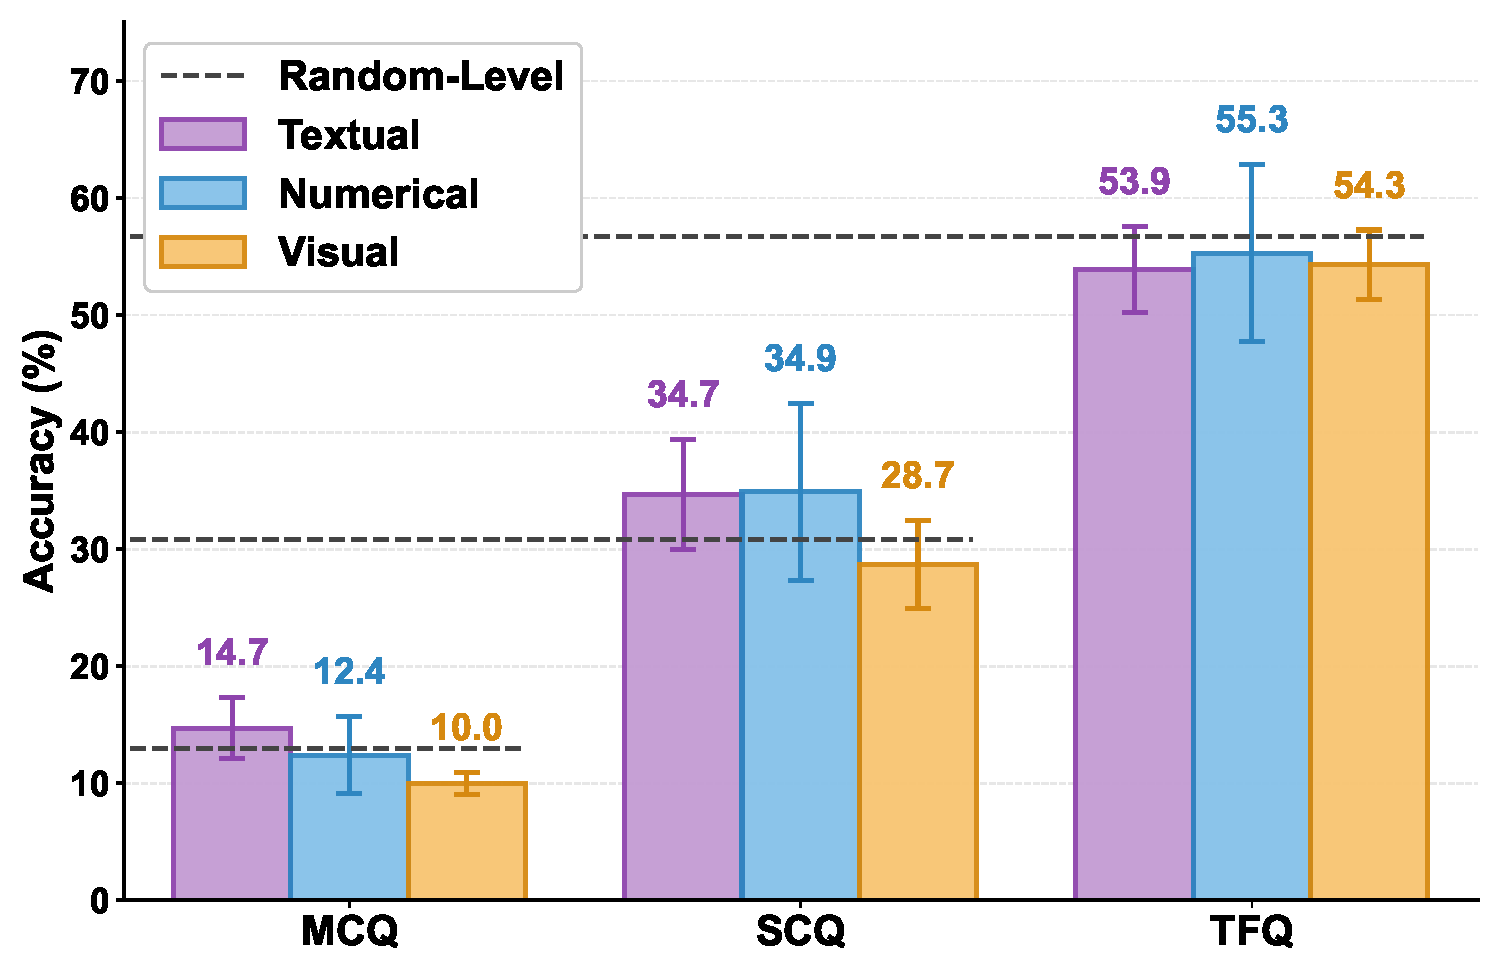
\includegraphics[width=\linewidth]{figure/figure20.pdf}
    \vspace{-5mm}
	\caption{Modality-Agnostic properties along with different models and different problem tasks.}
	\label{fig:cross-modality}
    \vspace{-5mm}
\end{figure}

\subsection{Insight of Capability Collapse}
\label{analysis}
1) \textbf{Complete performance crash.} 
It is widely accepted that the models we tested have represented the capability upper bound of current LLMs.
By contrast, GPT-5.4 scores a mere 8.60\% on MCQ, 26.80\% on SCQ, and 52.02\% on TFQ in the visual modality—falling strictly below the pure random guessing threshold across all three metrics.
Claude-4.6-opus exhibits a similarly dismal and comprehensive collapse (MCQ: 11.40\%, SCQ: 30.60\%, TFQ: 56.59\%).
Therefore, this perceived "ceiling" is now facing a \emph{catastrophic failure} under our evaluation framework across all task formats.
These empirical evidences reveal that these apex models would even fail to reach the mathematical upper probability of random chance, regardless of problem tasks.

2) \textbf{Incompatibility between architecture and physical world.}
More crucially, even within their native and most proficient textual modality, the performance of these top-tier models still remains fundamentally constrained. 
While GPT-5.4 and Claude-4.6-opus barely manage to cross the random baseline on textual MCQ and SCQ, they persistently fall below the baseline on TFQ (e.g., GPT-5.4: 54.23\%, Claude-4.6-opus: 53.54\%). 
Furthermore, they are comprehensively outperformed by the traditional lightweight LSTM architecture across the entire metric matrix (MCQ: 20.00\%, SCQ: 37.20\%, TFQ: 61.74\%).
This persistent cross-modal degradation intuitively proves that the capability collapse of LLMs on heterogeneous physical world tasks is not an accidental byproduct of format complexity or insufficient training.
On the contrary, it exposes that the entire \emph{autoregressive next-token prediction paradigm} itself inherently possesses an \emph{insurmountable capability ceiling}.



\begin{figure}[!t]
	\centering
	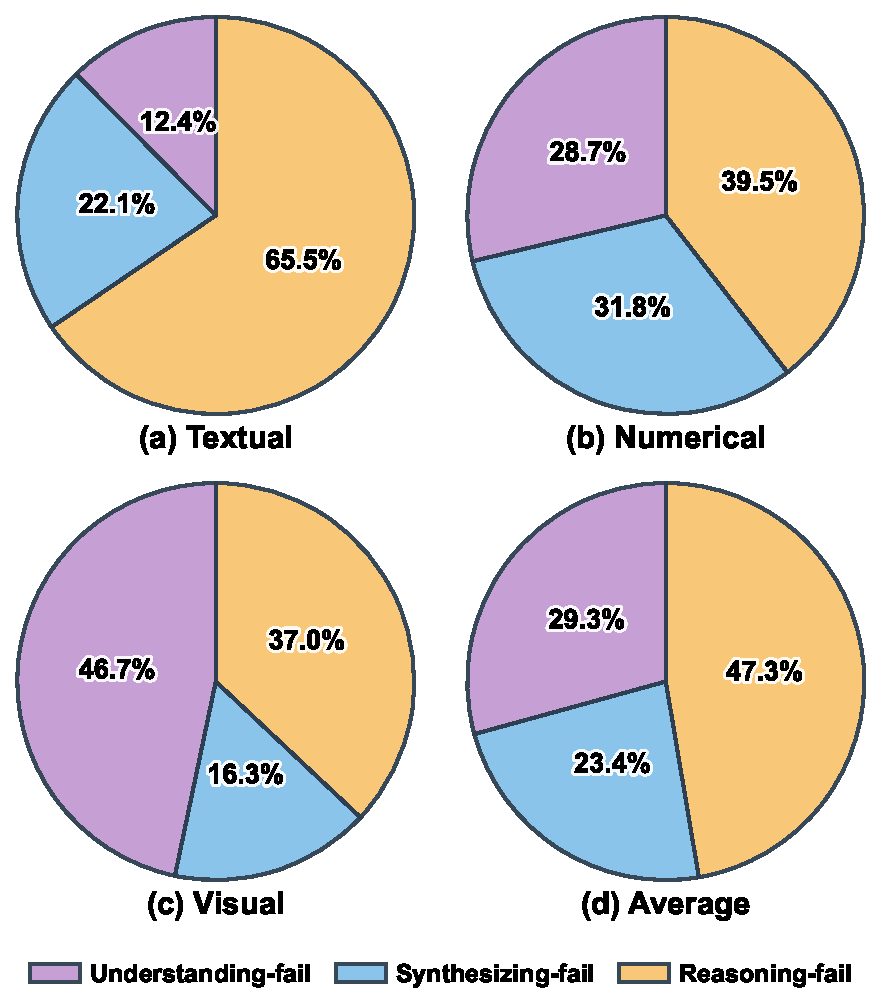
\includegraphics[width=0.90\linewidth]{figure/figure15.pdf}
	\caption{Error Attribution across the U/S/R Chain, exposing the fragility of High-Level Cognition in LLMs.}
	\label{fig:HCL}
\end{figure}

\section{Discussion}
\label{sec:discussion}

This section fundamentally and insightfully explores the underlying mechanisms of this collapse and its implications for future real Artificial General Intelligence (AGI). 

Specifically, we deconstruct the collapse into deficits across \textbf{three core characteristics}: 
(i) the \emph{violation of Modality-Agnosticism}, evaluated via cross-modal performance comparisons; 
(ii) the \emph{breakdown of High-Level Cognition}, analyzed through error attribution along the Understanding-Synthesizing-Reasoning (U/S/R) chain; 
and (iii) the \emph{absence of Open-ended Evolution}, demonstrated by contrasting general LMs, fine-tuned LMs, and traditional architectures. 
% Furthermore, we stress-test the models using few-shot learning to rule out shallow causes like insufficient context. 
Finally, we highlight the \textbf{evolutionary bottlenecks} in the current AGI trajectory and outline future directions.

\begin{figure}[!t]
	\centering
	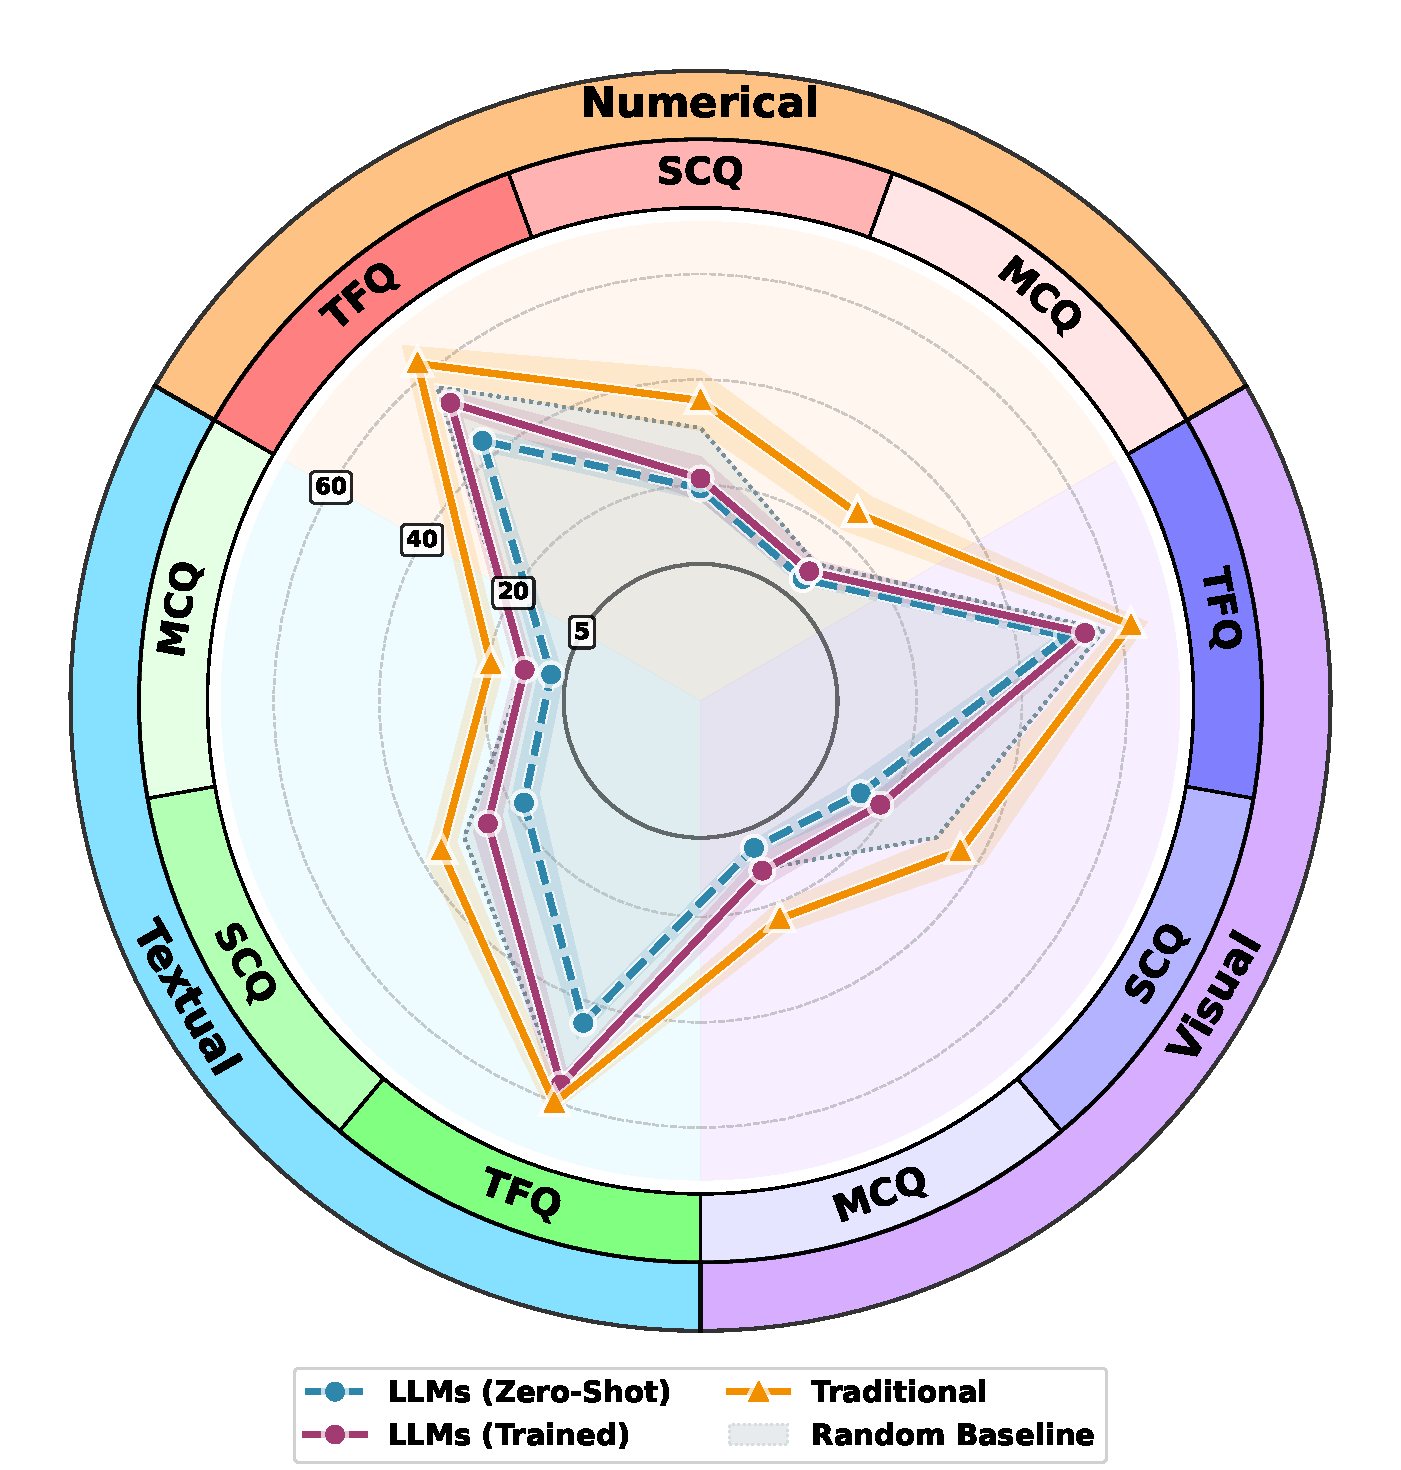
\includegraphics[width=\linewidth]{figure/figure18.pdf}
	\vspace{-5mm}
    \caption{Evaluation of Open-Ended Evolution comparing LLMs and traditional-architecture models across modalities.}
    \vspace{-4mm}
	\label{fig:evolution}
\end{figure}

\subsection{Modality-Agnosticism}
\label{modality}

To evaluate the \textit{Modality-Agnostic} capability, we analyze performance across different modalities with various problem tasks illustrated in Figure ~\ref{fig:cross-modality}. 

While elite models maintain a fragile reasoning facade in the textual modality, their cognitive capabilities catastrophically collapse in \emph{non-semantic environments}.
Remarkably, massive LLMs universally perform \emph{worse than random chance} across all metrics. 
The most glaring deficit occurs in the simplest binary task (TFQ, random baseline $56.74\%^\dagger$), where models like LLaVa-1.5 (Visual) and Vicuna-1.5 (Numerical) plunge to a mere $50.00\%$. 
As reasoning complexity increases, the capability gap widens to absurd proportions: on the visual MCQ, LLaVa-1.5 yields just $5.40\%$, and Llama-3.1 (70B) scores a dismal $6.40\%$ on the numerical MCQ. 
% Both scores are less than half the $12.95\%^\dagger$ random baseline. 
This multi-dimensional, sub-random collapse definitively proves that current LMs \textbf{lack genuine modality-agnosticism}; their reasoning is heavily tethered to textual semantic shortcuts, completely failing to integrate raw physical signals.
In stark contrast, specialized lightweight traditional-architecture models provide compelling empirical proof for representational equivalence. 
Despite processing radically different raw inputs, these models not only overwhelmingly crush their billion-parameter counterparts but also converge on nearly identical predictive distributions. 

This gap indicates that the next frontier of AGI is not simply scaling language priors, but \textbf{learning abstractions that remain invariant across how the world is observed}. 
If future models cannot reason consistently beyond text, then their apparent intelligence may remain a semantic illusion rather than genuine world intelligence.

% Whether utilizing a Textual GRU, a Numerical CNN, or a Visual EfficientNet-B0, their accuracies universally stabilize across the entire gradient: 
% peaking at $60\%$-$63\%$ on TFQ, $32\%$-$38\%$ on SCQ, and $19\%$-$25\%$ on MCQ. 
% This flawless tri-modal convergence confirms that objective physical truths are invariant to sensory channels. 
% It proves that once a model's architecture aligns with the physical world's structural logic, it can consistently extract identical macroscopic laws regardless of the data modality.

\begin{figure*}[!t]
	\centering
	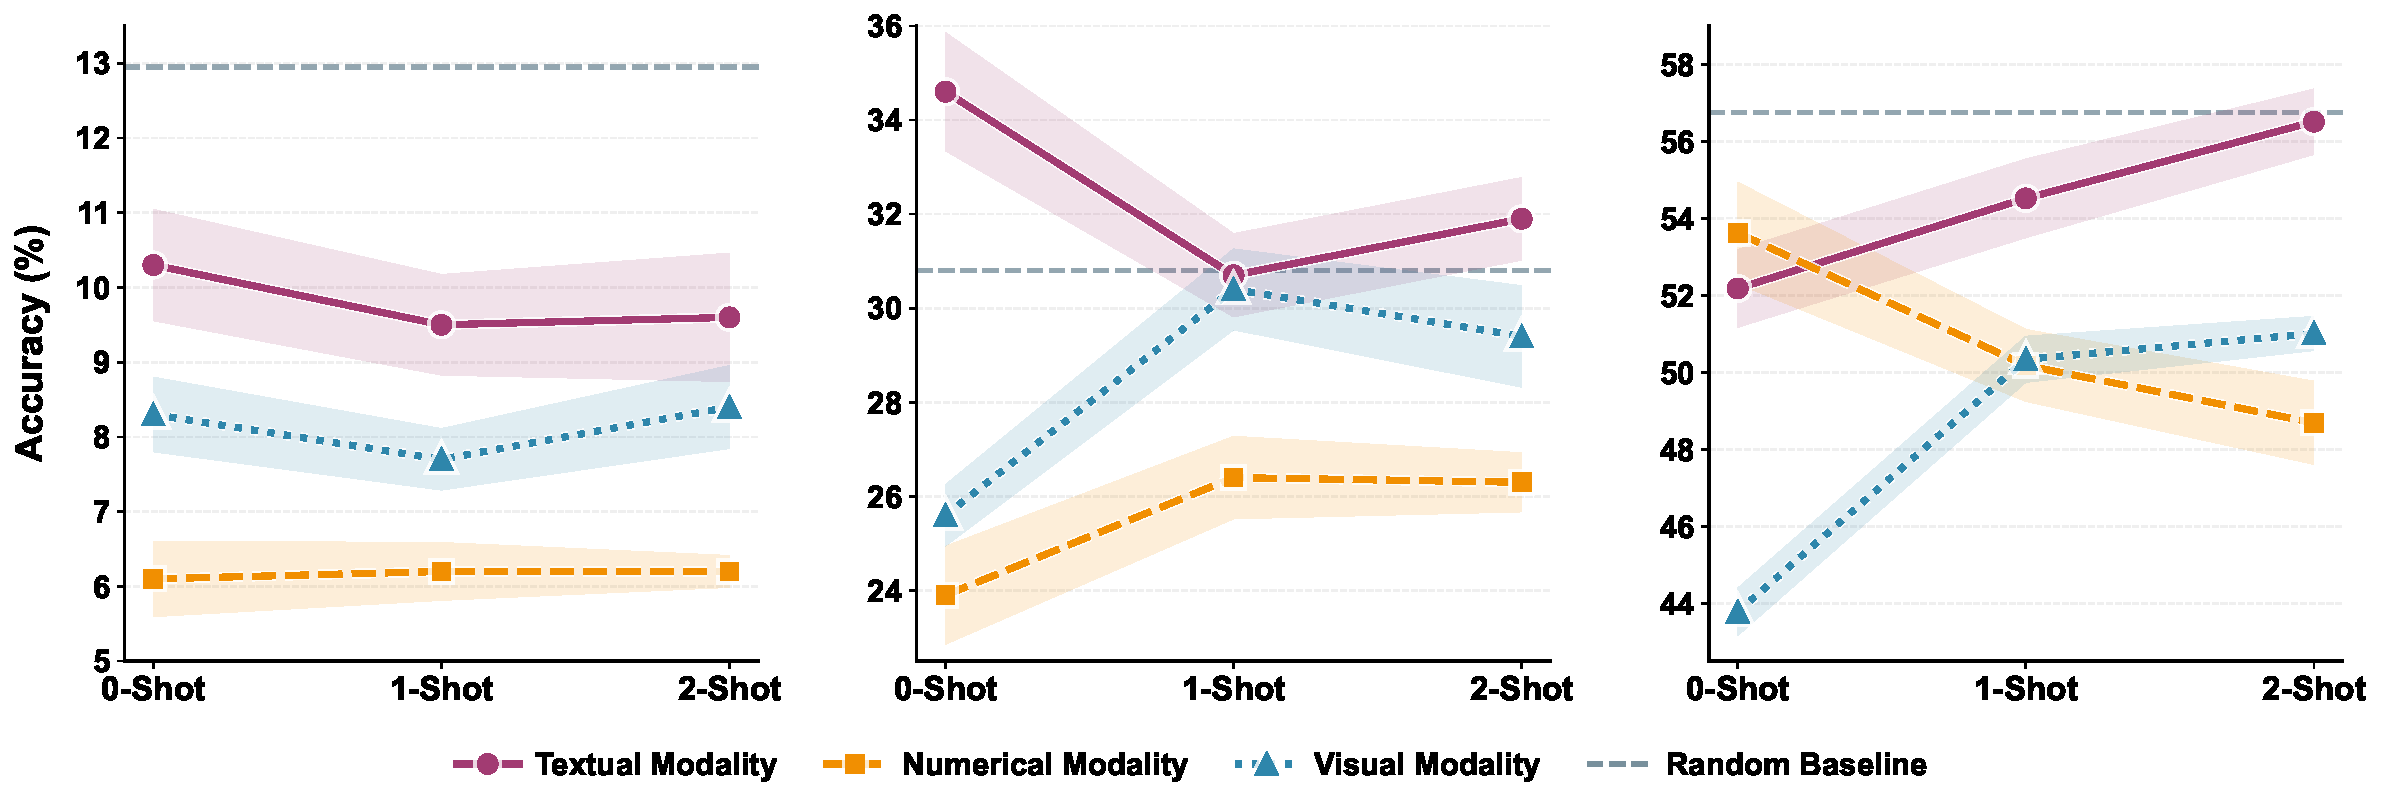
\includegraphics[width=\linewidth]{figure/figure16.pdf}
    \vspace{-5mm}
	\caption{Few-Shot Learning (FSL) Stress-Test. Accuracy trajectories across 0, 1, and 2-shot settings. Flat or degrading performance near random baselines indicates that FSL fails to trigger endogenous cognitive reasoning. (From left to right: MCQ, SCQ, TFQ)}
    \vspace{-2mm}
	\label{fig:few_shot_ablation}
\end{figure*}

\subsection{High-Level Cognition}
\label{HLC}

To gain deeper insight into the cognitive bottlenecks of High-Level Cognition for LLMs, we decompose each incorrect response by identifying its most probable point of failure within the U/S/R pipeline across modalities in Figure ~\ref{fig:HCL}, following the criteria detailed in Appendix~\ref{sec:usrules}. 

This diagnostic perspective serves as a vital complement to holistic accuracy: it reveals that models with comparable performance may nonetheless exhibit fundamentally distinct failure modes, exposing unique fractures along their internal cognitive chains. 
In the \emph{textual} modality, the majority of errors ($65.5\%$) are concentrated in the Reasoning stage. 
This suggests that while LLMs can maintain a facade of Understanding by adhering to output constraints (low U-fail), they lack the underlying world model to execute correct physical deduction. 
Meanwhile, as we shift to the \emph{numerical} and \emph{visual} modalities, we observe a surge in U-fail (reaching $46.7\%$ in visual tasks). 
This indicates that raw physical signals act as representational noise that disrupts the models' instruction-following stability, causing them to abandon the requested output formats entirely. 
Furthermore, the high S-fail in the \emph{numerical} modality ($31.8\%$) reflects a profound internal logical dissonance, where models simultaneously generate mutually exclusive physical states. 

These findings suggest that the next frontier for LLM research is not merely improving answer accuracy, but building models whose \textbf{cognitive pipelines remain structurally coherent} even when reasoning must emerge directly from raw world signals rather than semantic shortcuts.


\subsection{Open-Ended Evolution}
\label{evolution}
Facing specific physical-world problems, the training process of the model essentially serves as a mechanism to approximate the performance upper bound for a given task.

Empirical results in Figure ~\ref{fig:evolution} demonstrate that traditional architecture models establish a stable performance baseline through training, representing the physical upper bound of the \emph{passive fitting} capacity on specific data distributions within traditional AI paradigms. 
However, a compelling phenomenon emerges: 
despite undergoing equivalent training regimes, LLMs not only fail to surpass but comprehensively underperform compared to traditional architecture models. 
This performance therefore inversion exposes profound architectural limitations within LLMs: 
they are fundamentally incapable of efficiently achieving passive fitting to specific physical dynamics, even within closed environments. 

Following an a fortiori argument, Open-ended Evolution requires an intelligent agent to \textbf{continuously assimilate and reorganize knowledge} through active interaction with complex physical environments. 
If current LLMs fail even to reach the upper bound of passive fitting in closed settings, then their limitation is not merely insufficient training, but a more fundamental mismatch between next-token prediction and genuine cognitive evolution. 


\subsection{Exploration and Future Work}
\label{future}

To investigate whether the observed collapse partially stems from the lack of task-specific context, we conducted a rigorous stress-test using \textbf{Few-Shot Learning} (FSL) with 1-shot and 2-shot demonstrations. 
The empirical results reveal a profound stagnation in capability emergence. Despite providing explicit examples, model performance remains stubbornly tethered to the mathematical random baseline. 
% In the numerical modality, for instance, MCQ accuracy remained virtually frozen at approximately $6.20\%$. Most strikingly, in the textual modality, increasing demonstrations to 2-shot actually led to a marginal performance decline (from $10.30\%$ to $9.60\%$). 
Qualitative analysis of the error logs also confirms that while FSL marginally improves template compliance and reducing Understanding-fail pattern, it still fails to trigger any substantive reduction in Reasoning-fail pattern with exacerbated reasoning errors. 
To summarize, this decoupling proves that FSL in current LLMs provides only \textbf{surface-level alignment} instead of perceiving the underlying laws of the physical world. 

Taken together, the failures across \textbf{modality, cognition, and evolution} indicate that current LLMs are constrained by a \emph{paradigm that remains fundamentally text-bound, externally scaffolded, and passively optimized}. 
The next stage of AGI will therefore require a shift from scaling semantic prediction to building systems that can \emph{form unified world representations, maintain endogenous cognitive structure, and grow through real interaction}. 
Under this view, HWI defines a broader transition for the field: from language competence toward authentic world intelligence.

% In the absence of genuine physical logic, additional context acts as "semantic noise" that further destabilizes the model’s fragile reasoning. 
% This decoupling proves that FSL in current LLMs provides only surface-level alignment; it teaches the model how to output a response without enabling the structural cognitive required to perceive the underlying laws of the physical world. 
% Consequently, the persistence of sub-random performance across all shot settings exposes an insurmountable capability ceiling within the "autoregressive next-token prediction" paradigm. 
% These findings demonstrate that AGI cannot be realized through prompt engineering or scaling context alone; it necessitates a paradigm shift toward an endogenous, modality-agnostic architecture capable of autonomous, world-oriented synthesis.

\section{Conclusion}
\label{sec:conclusion}

In this work, we introduce \textbf{Holistic World Intelligence (HWI)} as a principled perspective for evaluating progress toward AGI, grounded in three core attributes: 
\emph{Modality-Agnosticism}, \emph{High-Level Cognition}, and \emph{Open-ended Evolution}. 
Through the proposed \textbf{WorldScope} benchmark and systematic analyses, we show that current state-of-the-art LLMs suffer a broad \emph{capability collapse} when reasoning must emerge from heterogeneous physical-world signals rather than textual semantics. 
These findings suggest that the central obstacle to AGI is no longer scaling language alone, but building systems that can internalize world-invariant structure, sustain endogenous cognitive organization, and improve through real interaction with the world.


%%
%% The next two lines define the bibliography style to be used, and
%% the bibliography file.
\clearpage
\bibliographystyle{ACM-Reference-Format}
\bibliography{sample-base}

\clearpage
% =============================================================================
% Appendix (MatchIntel2 / MHLC)
% Style inspired by ref.txt: overview index, Parts with \clearpage between them.
% =============================================================================

\section*{Appendix Overview}
\label{app:overview}

This appendix collects the detailed dataset formulation, experiment setup, case studies, limitations, and auxiliary rules referenced in the main paper. We organize the material into the following parts for navigation.

\paragraph{Part A: Detailed Dataset Formulation.}
\begin{itemize}
    \item \textbf{A.} Raw feature definitions (Appendix~\ref{app:raw_features}).
    \item \textbf{B.} The 12 playing-style labels (Appendix~\ref{app:twelve_styles}).
    \item \textbf{C.} Data statistics (Appendix~\ref{app:data_stats}).
    \item \textbf{D.} Construction pipeline (Appendix~\ref{app:construction_pipeline}).
\end{itemize}

\paragraph{Part B: Experiment Setup.}
\begin{itemize}
    \item \textbf{E.} Models: PEFT fine-tuning of LLMs and traditional architecture models trained from scratch (Appendix~\ref{app:models}).
    \item \textbf{F.} Parameters: generation, PEFT, and training-from-scratch settings (Appendix~\ref{app:parameters}).
    \item \textbf{G.} Zero-shot and few-shot prompt templates (Appendix~\ref{app:prompts_zeroshot_fewshot}).
\end{itemize}

\paragraph{Part C: Case Studies.}
\begin{itemize}
    \item \textbf{H.} Qualitative failure cases and representative examples (Appendix~\ref{app:Case Studies}).
\end{itemize}

\paragraph{Part D: Limitations \& Future Work.}
\begin{itemize}
    \item \textbf{I.} Limitations (Appendix~\ref{app:limitations}).
    \item \textbf{J.} Future work (Appendix~\ref{app:future_work}).
\end{itemize}

\paragraph{Part E: U/S/R Error Attribution (auxiliary).}
\begin{itemize}
    \item \textbf{K.} Rule-level definitions for U/S/R discussion and log-based attribution (Appendix~\ref{sec:usrules}).
\end{itemize}

% -----------------------------------------------------------------------------
% \clearpage

\section{Detailed Dataset Formulation}
\label{app:dataset_formulation}

\textbf{The necessity of constructing this dataset:} Existing multimodal datasets are still largely confined to low-level mechanical processing. Fundamentally, they map low-level inputs to other low-level outputs, making it difficult to evaluate whether LLMs can derive high-level conclusions by perceiving the underlying logic behind these data.

\textbf{The reliability of the data source:} This dataset is collected from WhoScored, a leading professional football analysis website. As an authoritative source widely used in sports analytics research \cite{li2022emergent,liu2025can,mahowald2024dissociating}, WhoScored relies on domain experts to maintain high-fidelity match annotations, making it a suitable source for evaluating HWI-related capabilities of LLMs.

\subsection{Raw Feature Definitions}
\label{app:raw_features}

\begin{figure}[!t]
	\centering
	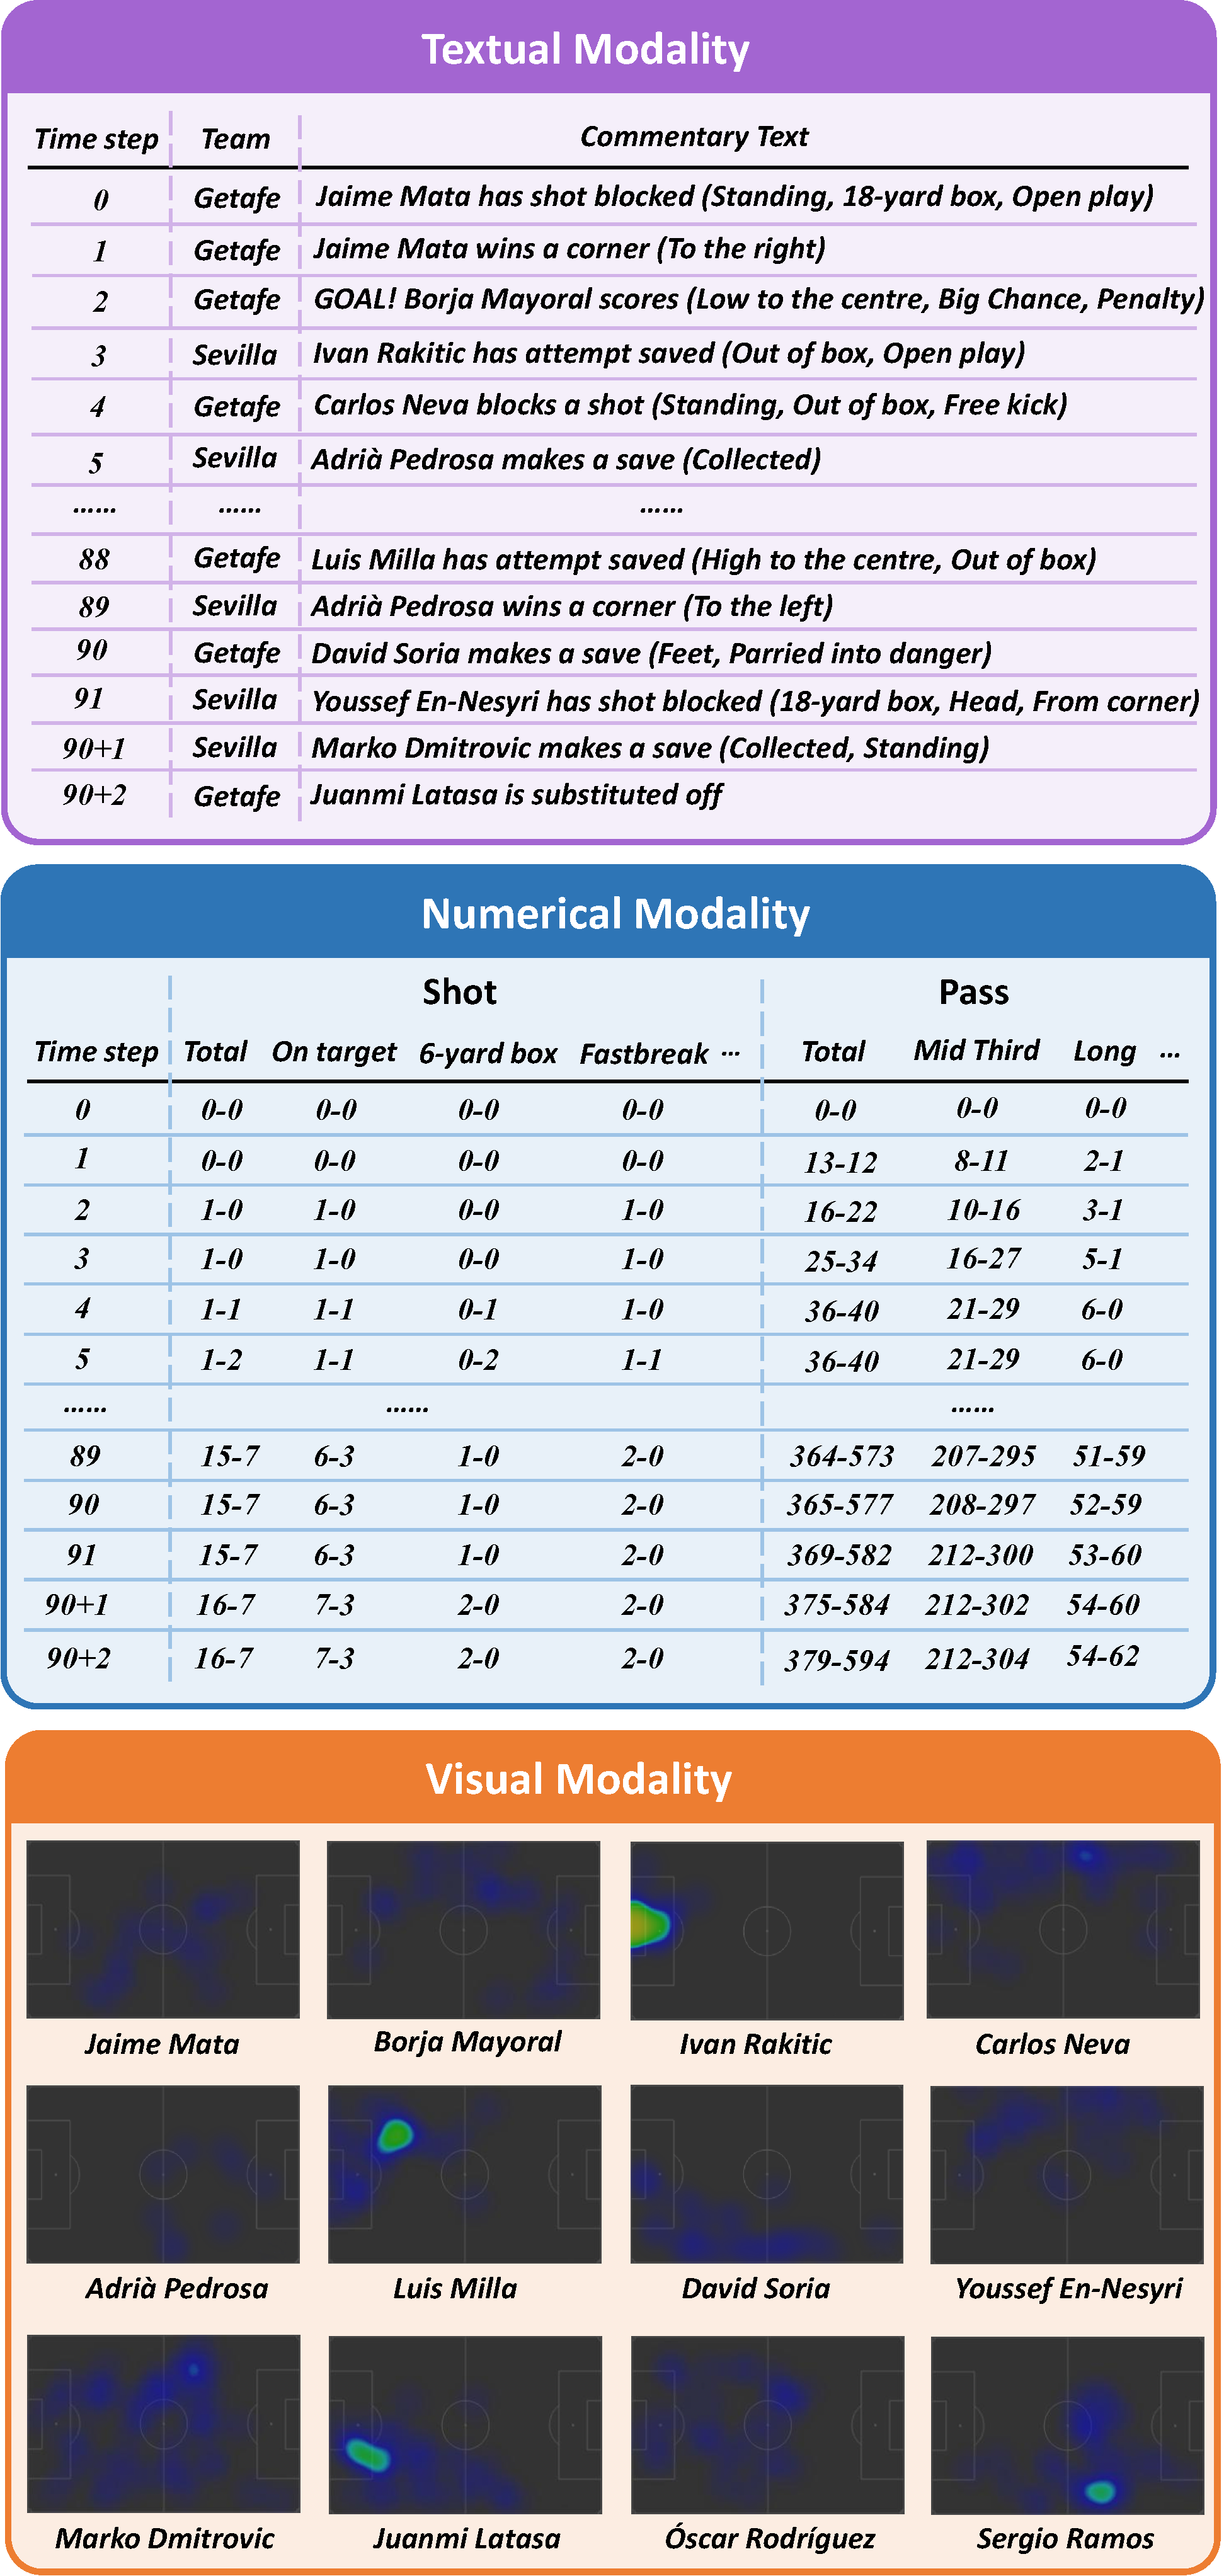
\includegraphics[width=\linewidth]{figure/ful2.pdf}
	\vspace{-5mm}
    \caption{Examples of three different modalities from a sample match.}
    \vspace{-4mm}
	\label{fig:data_introduction}
\end{figure}

WorldScope benchmark pairs low-level physical observations with high-level tactical style labels. All data are collected from the official website. \textbf{Textual modality:} We extract commentary texts from the \emph{Match Commentary} section of the \emph{Match Centre}. These texts provide descriptions of player actions (e.g., to the right, standing) and ball-related events (e.g., makes a save, wins a corner) at different time steps. \textbf{Numerical modality:} We extract fine-grained cumulative statistics at selected time steps from the \emph{Chalkboard} section of the \emph{Match Centre}. These metrics range from fundamental actions (e.g., passes and dribbles) to spatial and situational attributes (e.g., pitch zones and action direction). \textbf{Visual modality:} We collect positional heatmaps for all participating players from the \emph{Heatmaps} section of the \emph{Match Centre}, covering their spatial distribution over the full match. Figure~\ref{fig:data_introduction} illustrates an example from the three modalities.

These data are raw observations directly captured from the match and are therefore low-level in nature. Within each modality, individual data points are inherently fragmented: whether a single textual snippet, a discrete numerical update, or an isolated player heatmap, each observation remains only weakly interpretable in isolation. To overcome this, the model must integrate evidence across temporal and spatial dimensions within each modality to reconstruct the overall match narrative, rather than relying on simplistic single-feature shortcuts.

% A formal schema (field names, types, alignment with Match Centre exports, and normalization rules) will be inserted here when you finalize the release specification.

\subsection{The 12 Styles}
\label{app:twelve_styles}

The high-level outputs are directly extracted and unmodified from the \emph{Match Summary} section of the official \emph{Match Report}. Crucially, they are annotated by their domain experts, which eliminate any subjective bias or dataset tailoring. Through exhaustive data collection, we empirically verified that the platform's \textbf{domain experts annotate} matches using a closed set of exactly 12 discrete playing styles:

\textit{1). Played with width}

\textit{2). Favoured long shots}

\textit{3). Favoured short passing}

\textit{4). Attacked through the middle}

\textit{5). Favoured through balls}

\textit{6). Attacked down the left side}

\textit{7). Favoured crossing the ball}

\textit{8). Favoured long balls}

\textit{9). Had a high shot frequency when in possession}

\textit{10). Dominated possession}

\textit{11). Attacked down the right side}

\textit{12). Had a large quantity of possession in their opponent's half}

We explicitly define these 12 tactical styles as macroscopic targets because they represent latent strategic intentions rather than directly observable atomic events. None of these labels can be trivially extracted from a localized input occurrence or via superficial semantic shortcuts. Instead, correctly predicting any of these styles rigorously forces the model to execute the complete Understanding-Synthesizing-Reasoning (U/S/R) cognitive chain: First, in the Understanding (U) stage, the model must accurately ground isolated physical events, such as analyzing the efficiency of individual pass from numerical matrices or localized player densities from visual heatmaps. Next, in the Synthesizing (S) stage, it must integrate these fragmented, minute-by-minute atomic observations into a coherent, global spatial-temporal state—for instance, recognizing a persistent structural pattern where the ball is predominantly distributed along both flanks over the entire 90 minutes. Finally, in the Reasoning (R) stage, the model must transcend statistical counting to deduce the latent tactical philosophy, logically mapping this unified global dynamic to the specific strategic intentions.

% \textit{Played with width; Favoured long shots; Favoured short passing; Attacked through the middle; Favoured through balls; Attacked down the left side; Favoured crossing the ball; Favoured long balls; Had a high shot frequency when in possession; Dominated possession; Attacked down the right side; Had a large quantity of possession in their opponent's half}.

% Optional: per-label definitions, co-occurrence constraints, and annotation guidelines can be added in this subsection.

\begin{figure}[!t]
	\centering
	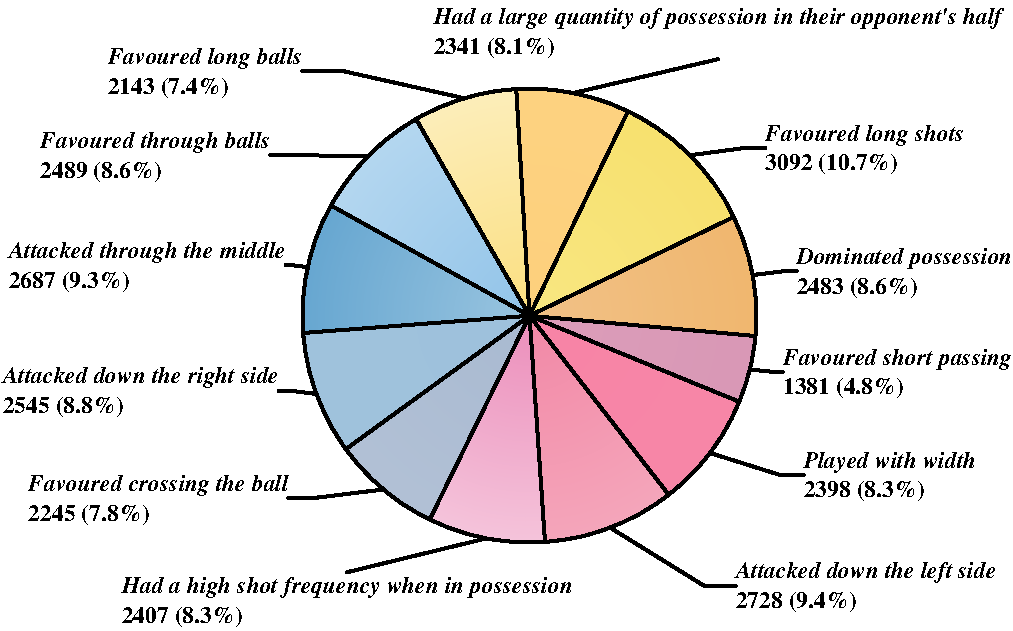
\includegraphics[width=\linewidth]{figure/new1.pdf}
	\vspace{-5mm}
    \caption{A pie chart showing the statistical data of playing styles in the dataset. It shows all the statements about playing styles, with their respective quantities and proportions.}
    \vspace{-4mm}
	\label{fig:evolution}
\end{figure}

\subsection{Data Statistics}
\label{app:data_stats}

Recordable matches from 2018 to 2023 were extracted via web crawling. During preprocessing, invalid records were identified and removed. For example, some matches contained incomplete commentary texts, missing statistical values, or lacked corresponding match reports. Importantly, this collection and filtering process is strictly architecture-agnostic. \textbf{We rely solely on automated web scraping and manual verification for data completeness, without any tailored feature engineering intended to favor models.} Furthermore, to ensure the semantic fidelity of the benchmark, we introduced a \textbf{rigorous human validation step}. Researchers familiar with football domain knowledge randomly sampled 20\% of the automatically filtered matches to manually verify the content quality—ensuring, for instance, that the scraped texts were genuine play-by-play commentaries rather than website artifacts, and that the multimodal observations logically corresponded to the annotated tactical styles. After this comprehensive cleaning and validation process, the final dataset contains complete records from 7 tournaments between 2018 and 2023. In total, 5,000 match records were retained and stored in JSON format. Unlike conventional multimodal datasets that often suffer from unbalanced modality distributions or missing paired data, WorldScope features strictly aligned cross-modal triplets. Specifically, each of the 5,000 match records is perfectly accompanied by all three heterogeneous inputs (textual commentary, numerical statistics, and visual heatmaps). This strict alignment results in 15,000 distinct input instances ($5,000 \times 3$ modalities) evaluated across the benchmark. Furthermore, these 5,000 holistic records are mapped onto the 12 expert-annotated tactical styles, offering a diverse and rich distribution of macroscopic targets for cognitive evaluation. This meticulously aligned scale and comprehensive label coverage provide a solid empirical basis for evaluating high-level cognition in models. We summarize the dataset scale in Table~\ref{fig:dataset_scale}.

% We summarize dataset scale and splits (e.g., train/test counts, per-modality coverage, label frequency, and sequence length statistics). \textbf{Placeholder:} insert tables or figures with your final numbers.

% \begin{table}[t]
%     \centering
%     \caption{Placeholder: MatchIntel2 statistics (splits, label distribution, sequence lengths, etc.).}
%     \label{tab:app_data_stats_placeholder}
%     \begin{tabular}{l c}
%         \toprule
%         \textbf{Statistic} & \textbf{Value (TBD)} \\
%         \midrule
%         Total examples & TBD \\
%         Train / Test split & 4{,}500 / 500 \\
%         Per-label frequency (12 styles) & TBD \\
%         Other (e.g., avg.\ timesteps per match) & TBD \\
%         \bottomrule
%     \end{tabular}
% \end{table}

% Table generated by Excel2LaTeX from sheet 'Sheet1'
\begin{table}[t]
  \centering
  \caption{Collection status of the dataset. The dataset covers 7 tournaments from 2018 to 2023.}
  \renewcommand\arraystretch{1.5} 
  \resizebox{\linewidth}{!}{
    \begin{tabular}{l|cccccc|c}
    \bottomrule
    \diagbox[width=15em,height=2.0em]{Tournaments}{Year} & 2018  & 2019  & 2020  & 2021  & 2022  & 2023  & Total \\
    \hline
    Premier League (England)     & 117 & 135 & 115 & 132 & 118 & 126 & 743 \\
    Serie A (Italy)              & 114 & 104 & 128 & 121 & 110 & 103 & 680 \\
    LaLiga (Spain)               & 141 & 116 & 118 & 120 & 108 & 117 & 720 \\
    Ligue 1 (France)             & 136 & 111 & 85  & 136 & 103 & 122 & 693 \\
    Bundesliga (Germany)         & 109 & 95  & 87  & 115 & 114 & 106 & 626 \\
    Brasileirão (Brazil)         & 146 & 141 & 103 & 187 & 137 & 147 & 861 \\
    Liga Profesional (Argentina) & 131 & 119 & 36  & 123 & 133 & 135 & 677 \\
    \hline
    Total                        & 894 & 821 & 672 & 934 & 823 & 856 & 5000 \\
    \toprule
    \end{tabular}%
    }
  \label{fig:dataset_scale}%
\end{table}%

\subsection{Construction Pipeline}
\label{app:construction_pipeline}

The construction of WorldScope follows a systematic data acquisition pipeline from the WhoScored platform. The strictly decoupled nature of the benchmark is inherent in the site's architecture, since the inputs and outputs are retrieved from independent functional modules:

\begin{itemize}[leftmargin=*]
    \item \textbf{Input Acquisition (Event-based):} The low-level multimodal data are crawled from the \textit{Match Centre} and \textit{Chalkboard} sections. These sections provide objective, real-time logs of the match (e.g., coordinate-based heatmaps, timestamped commentary, raw statistical counts, and player heatmaps). This information represents the raw physical process of the match.
    
    \item \textbf{Output Acquisition (Expert-based):} The high-level tactical labels are directly extracted from the \textit{Match Report} section. Unlike the raw objective logs, these reports provide macroscopic tactical evaluations generated post-match. Instead of parsing free-form summaries, we directly retrieve the explicitly identified ``Team Characteristics'', which are natively categorized by the platform into a finite set of 12 tactical playing styles.
\end{itemize}

To ensure rigorous evaluation, we maintain strict separation during crawling and pairing. The input features are restricted to \textit{what happened} (facts), while the output labels represent \textit{how it was played} (interpretations). By aligning these two independently crawled sources through Match IDs, we create a non-trivial gap between low-level observations and high-level conclusions, reducing the possibility of simple surface overlap.

% -----------------------------------------------------------------------------
% \clearpage
\section{Experiment Setup}
\label{app:experiment_setup}

\subsection{Models}
\label{app:models}
To comprehensively evaluate HWI-related capabilities and establish the empirical boundaries of both general intelligence and passive data fitting, we select a diverse and representative set of models. \textbf{Closed-Source State-of-the-Art Models:} To probe the current ceiling of commercial foundation models, we evaluate GPT-5.4 and Claude-4.6-opus. These models are accessed strictly via their official APIs and are tested across all three modalities. \textbf{Open-Weight LLMs:} For the textual and numerical modalities, we select prominent open-weight LLMs spanning various parameter scales to analyze potential scaling effects, including Llama-3.1 (70B), Mistral-Small-3 (24B), Qwen-2.5 (3B), and Vicuna-1.5 (7B). \textbf{Open-Weight VLMs:} To evaluate the visual modality, we utilize the corresponding multimodal variants of the aforementioned LLMs, namely Llama-3.2-Vision (90B), Mistral-Small-3.1 (24B), Qwen-2.5-VL (3B), and LLaVa-1.5 (7B). Crucially, the backbones of these VLMs are initialized from their corresponding text-only language models (e.g., Llama-3.2-Vision is built upon Llama-3.1, and Mistral-Small-3.1 is built upon Mistral-Small-3). This structural correspondence helps support a fairer cross-modal comparison when diagnosing the Modality Gap. Additionally, we fine-tune several representative LLMs on the training set, enabling a direct comparison against traditional architectures trained entirely from scratch. To ensure strict evaluation fairness across both training and inference stages, all models undergo rigorous \textbf{5-fold cross-validation} on the exact same data splits. This unified benchmarking guarantees that the observed performance gaps reflect genuine architectural capabilities rather than dataset bias. Full implementation and training details are provided below.

% This section consolidates model choices and training protocols referenced from Section~4. Hyperparameters are summarized in Appendix~\ref{app:parameters}.
\begin{figure*}[!t]
	\centering
	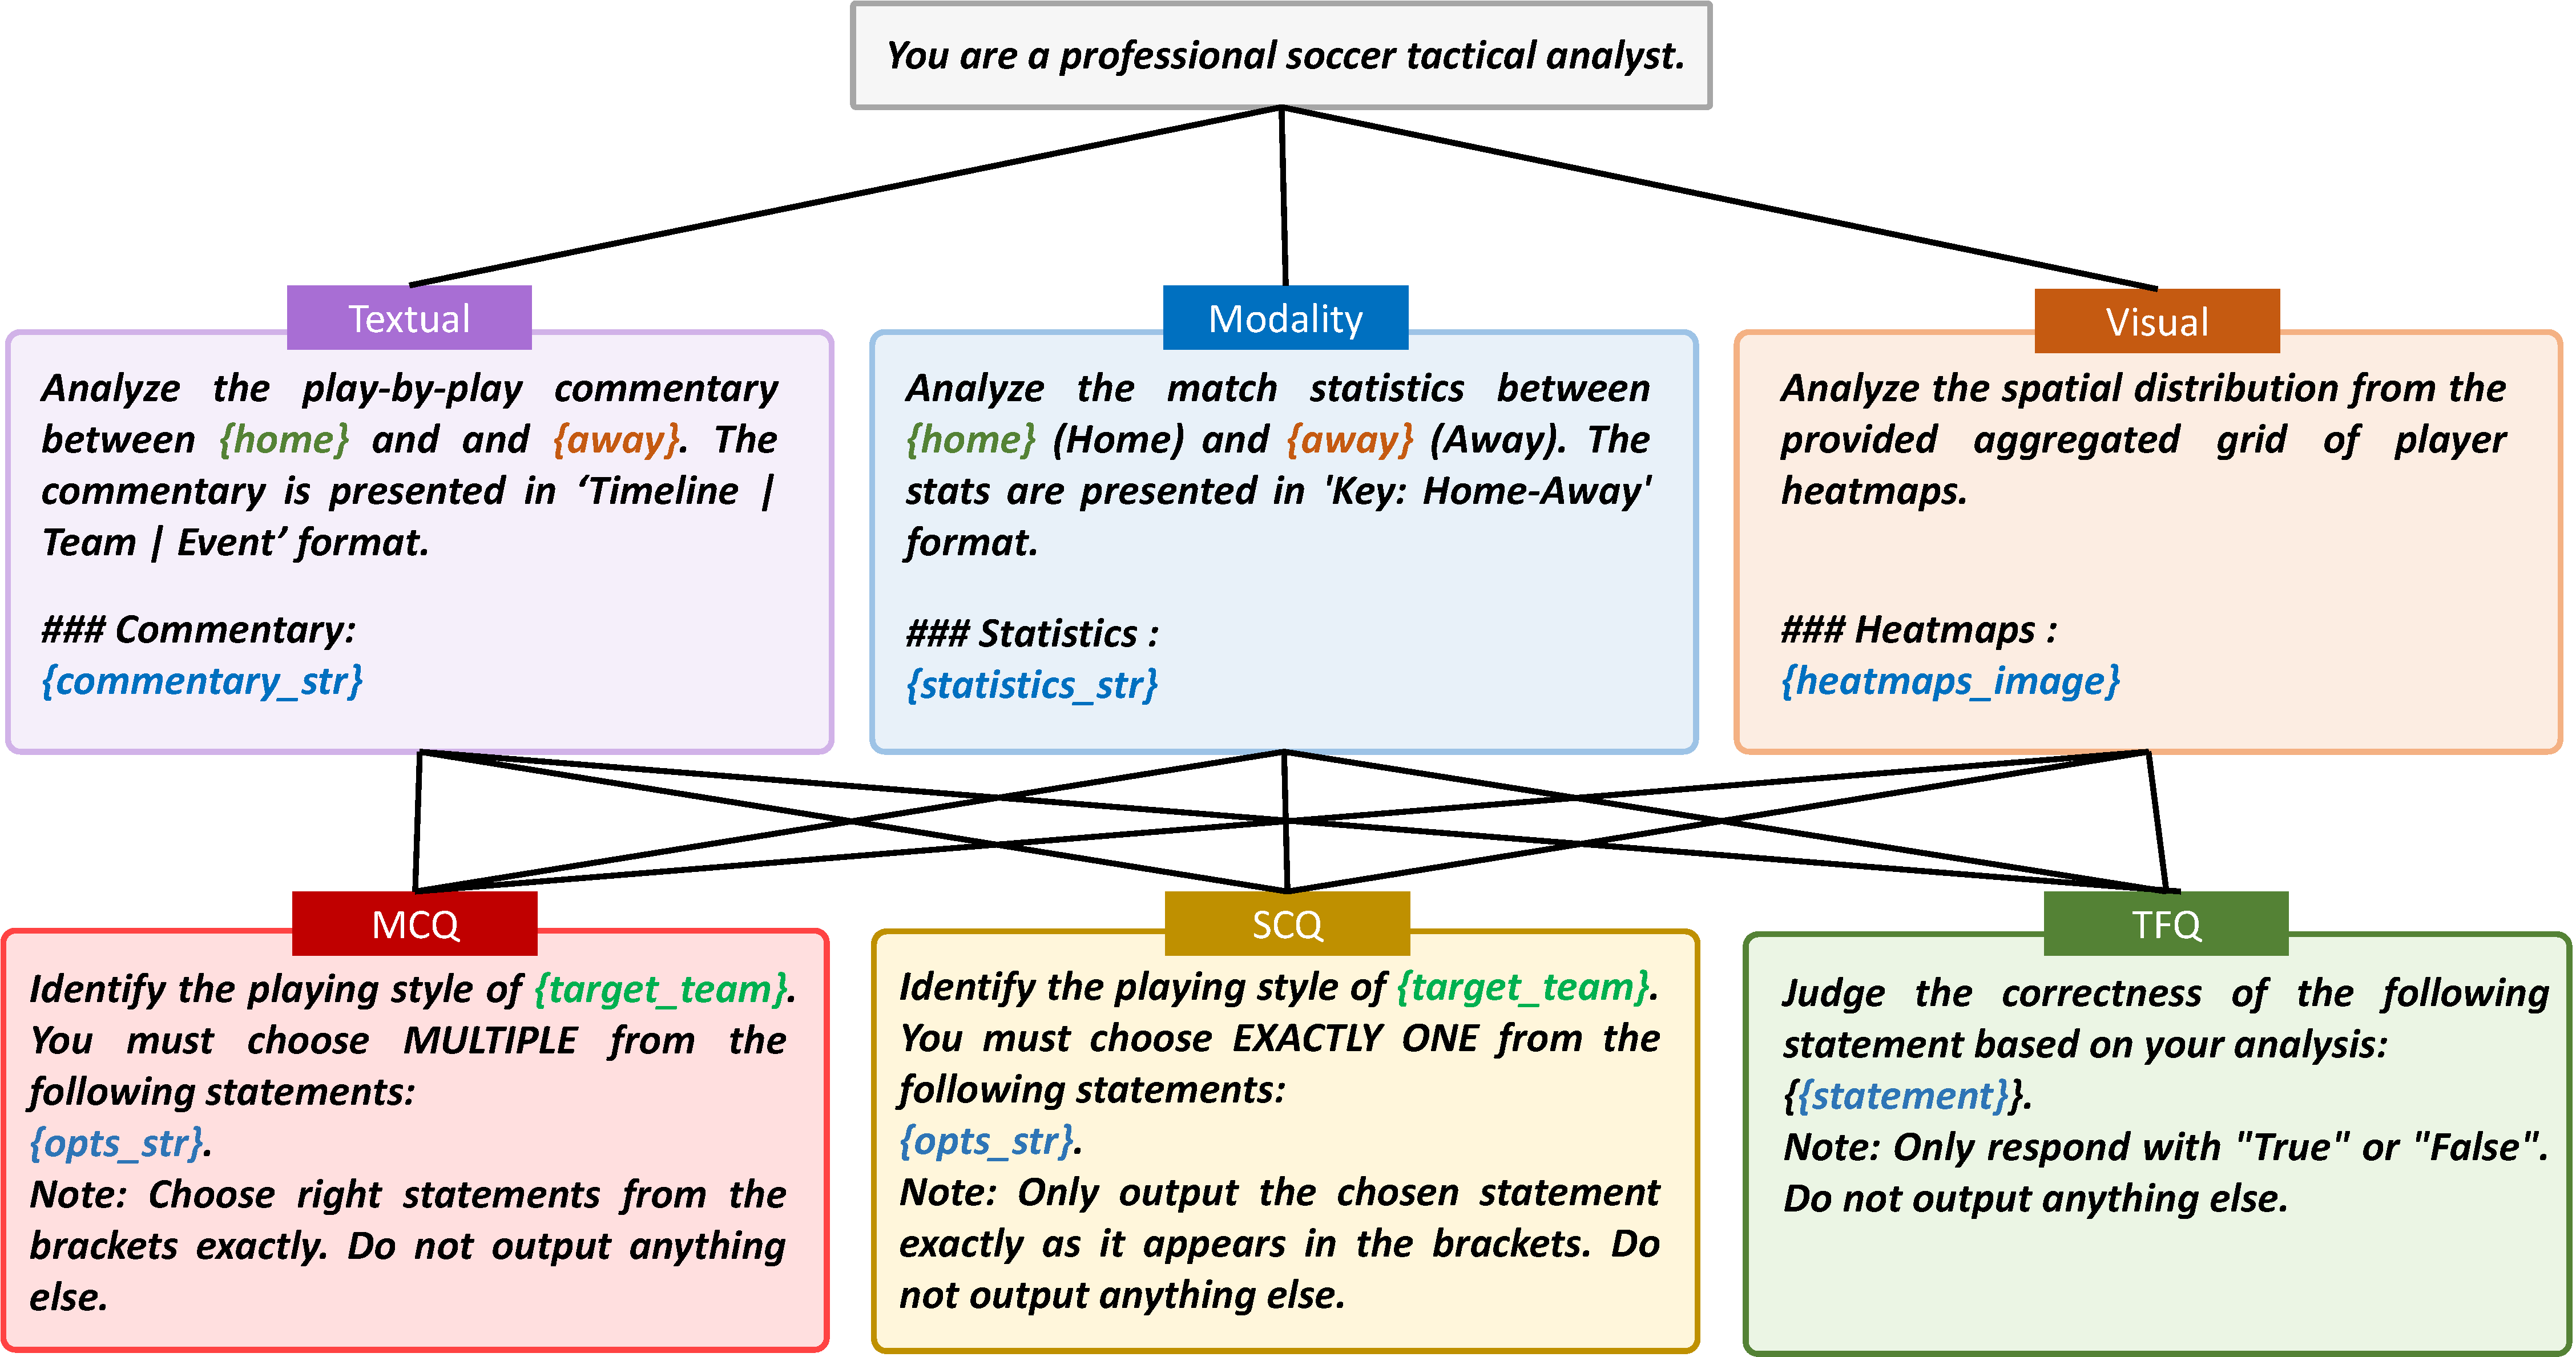
\includegraphics[width=\linewidth]{figure/figure23.pdf}
	\vspace{-5mm}
    \caption{Prompt design. First, the model is assigned the role of a soccer tactical analyst. Then, a task with a specified modality is provided, followed by a question in a specified format.}
    \vspace{-4mm}
	\label{fig:prompt}
\end{figure*}

\subsubsection{Fine-Tuning LLMs}
To adapt LLMs to the task, supervised fine-tuning (SFT) is performed on the collected dataset. Several models with strong instruction-following capabilities, specifically Qwen2-VL-2B, LLaVA-1.5-13B, Vicuna-13B-v1.5, and Qwen2.5-7B, serve as the foundation models across different modalities. To align with their input paradigms, the inputs are integrated into a unified conversational template. Specifically, for the visual modality, heatmaps are projected into the embedding space by vision encoders and aligned with fixed token placeholders, while fragmented numerical statistics are serialized into structured text for the textual and numerical modalities. This design allows LLMs to process the raw physical observations as conditional prefixes.

Additionally, to enable efficient fine-tuning, we adopt Quantized Low-Rank Adaptation (QLoRA). The foundation models are quantized to 4-bit precision using NormalFloat4 (NF4) with bfloat16 as the compute data type, and learnable Low-Rank Adapters (LoRA) are inserted into their linear projection layers, including both attention and MLP modules. During fine-tuning, the pre-trained weights remain frozen, and only the adapter parameters are updated through backpropagation. Training follows the standard causal language modeling paradigm, where models are trained to autoregressively generate high-level conclusions. The optimization minimizes the cross-entropy loss between the generated outputs and the ground-truth labels, strictly conditioned on the multimodal instruction context, with prompt tokens explicitly masked out from the loss.

\subsubsection{Training Traditional Architecture Models}
We train a suite of traditional architecture models to serve as rigorous baselines. These models bypass language-centric tokenization and process raw physical observations directly, aiming to predict the multi-label tactical styles of the target team.

For the textual modality, we introduce an event-driven framework to process the chronological play-by-play commentary. Each commentary event is tokenized and mapped to learned word embeddings. To handle varying sentence lengths, a masked average pooling mechanism is applied to extract a dense semantic representation for each text snippet. This textual feature is then concatenated with event-specific metadata, namely the normalized timestamp and binary team attribution, to construct a unified event vector that grounds the isolated text in the overall match context. To establish robust baselines, we independently train and evaluate three separate models on these sequences. The first, a pure Multi-Layer Perceptron (MLP), aggregates all events within a match via average pooling to form a global representation. In parallel, two bidirectional sequence models, GRU and LSTM, are trained individually to trace the chronological progression and contextual evolution of the match. These temporal models apply max pooling across the sequence dimension to extract the most decisive textual highlight signals associated with high-level tactical intents.

For the numerical modality, we design three distinct architectures to process the statistical data. The first is a hierarchical 1D Convolutional Neural Network (1D CNN) consisting of three consecutive convolutional blocks with batch normalization and ReLU activation, progressively expanding channel dimensions to extract local short-term dependencies from the sequential statistics. The second is a Delta-GRU model, which computes discrete differences across sequential milestones to capture the temporal evolution of match statistics. These dynamic variations are processed through a bidirectional Gated Recurrent Unit (GRU) and aggregated via a dual-pooling mechanism that concatenates adaptive average pooling and max pooling. The third is a pure Multi-Layer Perceptron (MLP) baseline that directly flattens the multi-step feature sequences into a unified vector. For all three architectures, the final aggregated representations are fed into a fully connected classifier to map the extracted patterns to multi-label predictions.

For the visual modality, we formulate the task as a Multiple Instance Learning (MIL) problem, where a complete match is treated as a bag of sequential heatmaps representing spatial activity zones over time. To comprehensively evaluate visual feature extraction, we employ three distinct shared instance-level encoders: ResNet-18, DenseNet-121, and EfficientNet-B0. Each backbone projects individual heatmap instances into high-dimensional feature vectors. Subsequently, a permutation-invariant max-pooling operation is applied across the instance dimension to aggregate these features into a unified representation. This design ensures that the most decisive signals for high-level outcomes can be retained without dilution, regardless of the specific time step at which they occur. The aggregated representation is then passed through an MLP classification head.

Finally, all traditional architecture models across the three modalities are optimized using binary cross-entropy loss.


\subsection{Parameters}
\label{app:parameters}

\subsubsection{Fine-Tuning Details and Hyperparameters}
LLMs are fine-tuned using 4-bit QLoRA ($r=64$, $\alpha=16$) for 5 epochs with the 32-bit Paged-AdamW optimizer. To accommodate the distinct characteristics of different modalities, hyperparameters are tailored accordingly: for visual tasks, the learning rate is set to $1\times10^{-4}$ with a dropout rate of 0.05 and a weight decay of 0.01; for numerical and textual tasks, the learning rate is $2\times10^{-4}$ with a dropout rate of 0.1 and a weight decay of 0.001. All models are trained with a warmup ratio of 0.03, a per-device batch size of 1, 8 gradient accumulation steps, and bfloat16 (BF16) precision.

% \subsubsection{Trained-from-Scratch Parameters}

\subsubsection{Implementation Details and Hyperparameters}
The traditional architecture models are optimized using the Adam optimizer and Binary Cross-Entropy (BCE) loss across all modalities. \textbf{Textual Modality:} The \texttt{bert-base-uncased} tokenizer is employed to process the commentary texts. To standardize the inputs, the sequences are capped at a maximum of 150 events per match and 32 words per event, with an embedding dimension of 128. These textual models are trained with a batch size of 16 and a learning rate of $10^{-3}$. \textbf{Numerical Modality:} Statistical sequences are constructed using 15-minute milestone intervals. All numerical architectures are trained with a batch size of 32 and an initial learning rate of $10^{-3}$, modulated by a cosine annealing learning-rate scheduler to ensure stable convergence. \textbf{Visual Modality:} Input heatmaps are resized to $215 \times 329$, with each MIL bag containing up to 18 instances representing the match evolution. To accelerate training while maintaining numerical stability, Automatic Mixed Precision (AMP) is employed. All visual models are optimized with a learning rate of $10^{-4}$.

\subsubsection{Inference Hyperparameters of LLMs}
To ensure stable generation of valid answers, we adopt nearly deterministic decoding settings. Specifically, the temperature is set to $10^{-4}$ and top-$p$ is set to 1.0.



\subsection{Prompt Design}
\label{app:prompts_zeroshot_fewshot}

For zero-shot evaluation, we design fixed instruction templates for each modality to help the language models interpret the distinct data formats and evaluate the task without cross-modal interference. Crucially, to verify model interface compatibility, we conducted a pre-task comprehension sanity check before the formal evaluation. When fed raw isolated inputs without downstream QA tasks and prompted to simply describe them, the evaluated LLMs and VLMs successfully identified the data structures (e.g., explicitly describing a visual input as a football player's positional heatmap or a text sequence as match commentary). This confirms that the models possess the fundamental capability to parse these low-level physical representations, thereby guaranteeing that our benchmark genuinely evaluates their endogenous cognitive abilities rather than mere interface incompatibility. \textbf{Textual Modality:} The context provides play-by-play commentary structured in a strictly chronological \texttt{Timeline | Team | Event} format. This sequential structure preserves the temporal dynamics of the match, enabling the model to trace tactical shifts and game momentum over time. \textbf{Numerical Modality:} The context presents time-series match statistics aggregated at specific milestones. The data are serialized into a structured \texttt{Key: Home-Away} format, allowing the model to directly quantify comparative team performance and event frequencies from discrete numerical indicators. \textbf{Visual Modality:} The model is instructed to evaluate spatial distributions derived from an aggregated grid of individual player heatmaps. This visual prompt encapsulates complex player activities into a single image, guiding the vision encoder to focus on spatial relationships and zonal dominance.

\textbf{Robustness via Diverse Task Formulations:} Following the modality-specific context, a standardized task query is appended. To rigorously evaluate the robustness of the models' cognitive capabilities and ensure that their performance is not an artifact of prompt engineering, we dynamically construct three distinct evaluation formats for \textit{each} test sample: 

\begin{itemize}
    \item \textbf{MCQ (Multiple-Choice Question):} Extract two to four appropriate playing styles from four candidates.
    \item \textbf{SCQ (Single-Choice Question):} Select one correct playing style from four candidates.
    \item \textbf{TFQ (True/False Question):} Judge whether a presented style set is absolutely correct.
\end{itemize}

By exposing the exact same physical sample to multiple heterogeneous question formats, we strictly test the models' robustness. A model possessing genuine high-level cognition must demonstrate consistent tactical deduction regardless of how the inquiry is formulated. To facilitate automated evaluation, these task queries require the model to output only deterministic answers (e.g., the exact option string or a boolean value). The prompts are shown in Figure~\ref{fig:prompt}. For few-shot learning, 1 to 2 high-quality demonstration examples are appended before the final query. Each demonstration pairs the corresponding intra-modality context with its reasoning process and final answer, thereby guiding the model's output distribution toward the expected response format through in-context learning.


% \subsection{Zero-Shot and Few-Shot Prompt}
% \label{app:prompts_zeroshot_fewshot}

% Zero-shot evaluation uses fixed instruction templates aligned with prior textual HLC work, with commentary replaced by numerical or visual inputs. Few-shot variants append 1--2 demonstration examples before the query. \textbf{Placeholder:} paste full prompt templates (per modality and per assessment format) here for reproducibility.


% Lightweight models are trained from scratch. The 1D CNN employs the Adam optimizer (lr=$10^{-3}$, kernel sizes $\{3, 5, 7\}$), and MIL-ResNet-18 processes the heatmaps (up to 18 images) using an ImageNet-pretrained backbone.

% -----------------------------------------------------------------------------
% \clearpage
\section{Case Studies}
\label{app:Case Studies}
This section presents several typical case studies to provide an deep analysis of the limitations of  LLMs in handling high-level cognition tasks. These cases cover errors in three representative reasoning tasks (MCQ, SCQ, TFQ), as well as severe failure scenarios such as generating completely irrelevant text. Figure \ref{fig:failure1}\textasciitilde \ref{fig:failure4} illustrate these failure patterns.
% \subsection{Models}
% \label{app:models}



% \subsection{Per-Class Accuracy}
% \label{app:per_class_accuracy}

% \textbf{Placeholder:} report per-style precision/recall or accuracy breakdown (e.g., macro-F1 per label) for each model family and modality.

% \begin{table}[t]
%     \centering
%     \caption{Placeholder: per-class metrics (12 styles $\times$ models).}
%     \label{tab:app_per_class_placeholder}
%     \begin{tabular}{l c c c}
%         \toprule
%         \textbf{Style / Model} & \textbf{Num.} & \textbf{Vis.} & \textbf{Notes} \\
%         \midrule
%         \multicolumn{4}{c}{\textit{TBD}} \\
%         \bottomrule
%     \end{tabular}
% \end{table}

% \subsection{Qualitative Case Study}
% \label{app:case_study}



% -----------------------------------------------------------------------------
% \clearpage
\section{Limitations \& Future Work}
\label{app:limitations_future}
\label{sec:limitations}

\subsection{Limitations}
\label{app:limitations}

Although this work provides critical insights into the capability boundaries of current large models, it is still subject to several limitations. First, while our zero-shot evaluations benchmark models with sizes up to 90B parameters, our fine-tuning experiments are constrained by computational resources and therefore focus on open-weight models up to 13B parameters. Although this scale is already sufficient to reveal the lack of endogenous structural growth in current LLMs under our setting, extending dynamic training to hundred-billion-parameter scales could further clarify the extreme boundaries of the observed Modality Gap. 

Second, to operationalize the HWI framework, the current WorldScope benchmark instantiates physical-world observations through three discrete channels: textual, numerical, and visual. However, the physical world inherently contains richer and more continuous signals, such as audio and temporal sensorimotor streams, which remain outside the scope of the present study. 

Third, to rigorously isolate and diagnose Modality-Agnostic properties, our current protocol evaluates the U/S/R cognitive chain by integrating fragmented data strictly within a single modality at a time. As a result, the more challenging setting of simultaneous cross-modality integration is not addressed in the current version of the benchmark.

\subsection{Future Work}
\label{app:future_work}

Addressing these limitations forms the trajectory of our future research. First, we plan to expand WorldScope into a more comprehensive benchmark that covers a broader spectrum of non-semantic and continuous physical modalities. Second, we will extend the current cognitive evaluation pipeline from single-modality reasoning to more complex cross-modality fusion, testing whether models can synthesize disjoint local states from heterogeneous channels into a unified global representation. 

Finally, to move beyond the capability collapse associated with passive data-fitting paradigms, we will explore the integration of specialized inductive biases and neuroplasticity-inspired architectures into LLMs. Ultimately, our goal is to equip foundation models with the capacity for authentic U$\rightarrow$S$\rightarrow$R cognition and sustained Open-ended Evolution, reducing their reliance on textual semantic shortcuts and bringing them closer to genuine world-grounded intelligence.

% \subsection{Limitations}
% \label{app:limitations}

% Constrained by available computational resources, fine-tuning focuses on open-weight models with parameter sizes up to 13B. These results support the absence of reliable MHLC in general LMs under our protocol, but larger scales could further validate the modality gap. The evaluation is conducted in numerical and visual modalities as representatives of non-semantic features; many physical-world signals (e.g., audio, sensorimotor streams) remain outside this study.

% \subsection{Future Work}
% \label{app:future_work}

% We plan to expand the evaluation framework into a broader non-semantic benchmark and to explore integrating specialized inductive biases into large-scale models so that U$\rightarrow$S$\rightarrow$R cognition can be realized without relying on textual semantic shortcuts.

% -----------------------------------------------------------------------------
% \clearpage
\section{U/S/R Error Attribution Rules}
\label{sec:usrules}

To move beyond the limitations of holistic performance metrics and provide a more granular diagnosis of model capabilities, we propose a systematic error-attribution protocol. Inspired by recent diagnostic methodologies that use rule-based verification frameworks to trace logical bottlenecks in language models \cite{mukherjee2026red,rafailov2023direct,zhiren2026learning}, we formalize the evaluation of the Understanding--Synthesizing--Reasoning (U/S/R) chain. Rather than relying on opaque heuristics, our protocol maps incorrect predictions to specific cognitive fractures using deterministic, bottom-up criteria derived from the model's raw output behavior:

\textbf{Understanding (U) Failure: Instruction Adherence and Grounding Collapse.} This foundational error is triggered when the model fails to extract the basic task semantics or to adhere to the explicitly specified output constraints. In our framework, the prompt strictly restricts the output to a predefined space of 12 tactical styles. A \textbf{U-fail} is recorded if the model generates unparseable text, conversational filler that violates the required format, or labels outside the candidate set. Such behavior indicates a fundamental collapse at the perception and grounding stage: the model is overwhelmed by the fragmented inputs and fails to recognize even the basic boundaries of the task.

\textbf{Synthesising (S) Failure: Internal Logical Dissonance via Mutual Exclusivity.} If the model successfully adheres to the output format and selects labels from the valid candidate set (thus passing the U stage), we then evaluate its internal consistency. Among the 12 tactical styles, certain subsets correspond to fundamentally contradictory physical states in football dynamics. For instance, a model that predicts both \textit{Favoured short passing} and \textit{Favoured long balls}, or simultaneously outputs \textit{Attacked through the middle} and \textit{Played with width}, exhibits a clear logical conflict. An \textbf{S-fail} is therefore assigned when the generated output contains such mutually exclusive label pairs. This indicates that, although the model can parse local events, it fails to synthesize them into a coherent and non-contradictory global interpretation.

\textbf{Reasoning (R) Failure: High-Level Semantic Misalignment.} The final stage of attribution occurs when the model produces an internally consistent and properly formatted output (passing both the U and S stages), yet the predicted tactical styles do not match the expert-annotated ground truth. An \textbf{R-fail} therefore isolates the error to the highest cognitive level. It indicates that the model is capable of perceiving the raw data and constructing a logically coherent scenario, but lacks the domain-specific reasoning ability required to map this synthesized world state to the correct macroscopic tactical conclusion.

\textbf{Implementation Details.} During evaluation, the model's raw output string is first parsed using regular expressions to match the 12 predefined style strings. The resulting predictions are then passed through an automated diagnostic pipeline: checking format adherence at the U stage, validating against a predefined matrix of mutually exclusive style pairs at the S stage, and finally comparing against the ground-truth labels via Exact Match at the R stage. This strict cascade ensures that the error attribution is mutually exclusive and collectively exhaustive.



\begin{figure*}[!t]
	\centering
	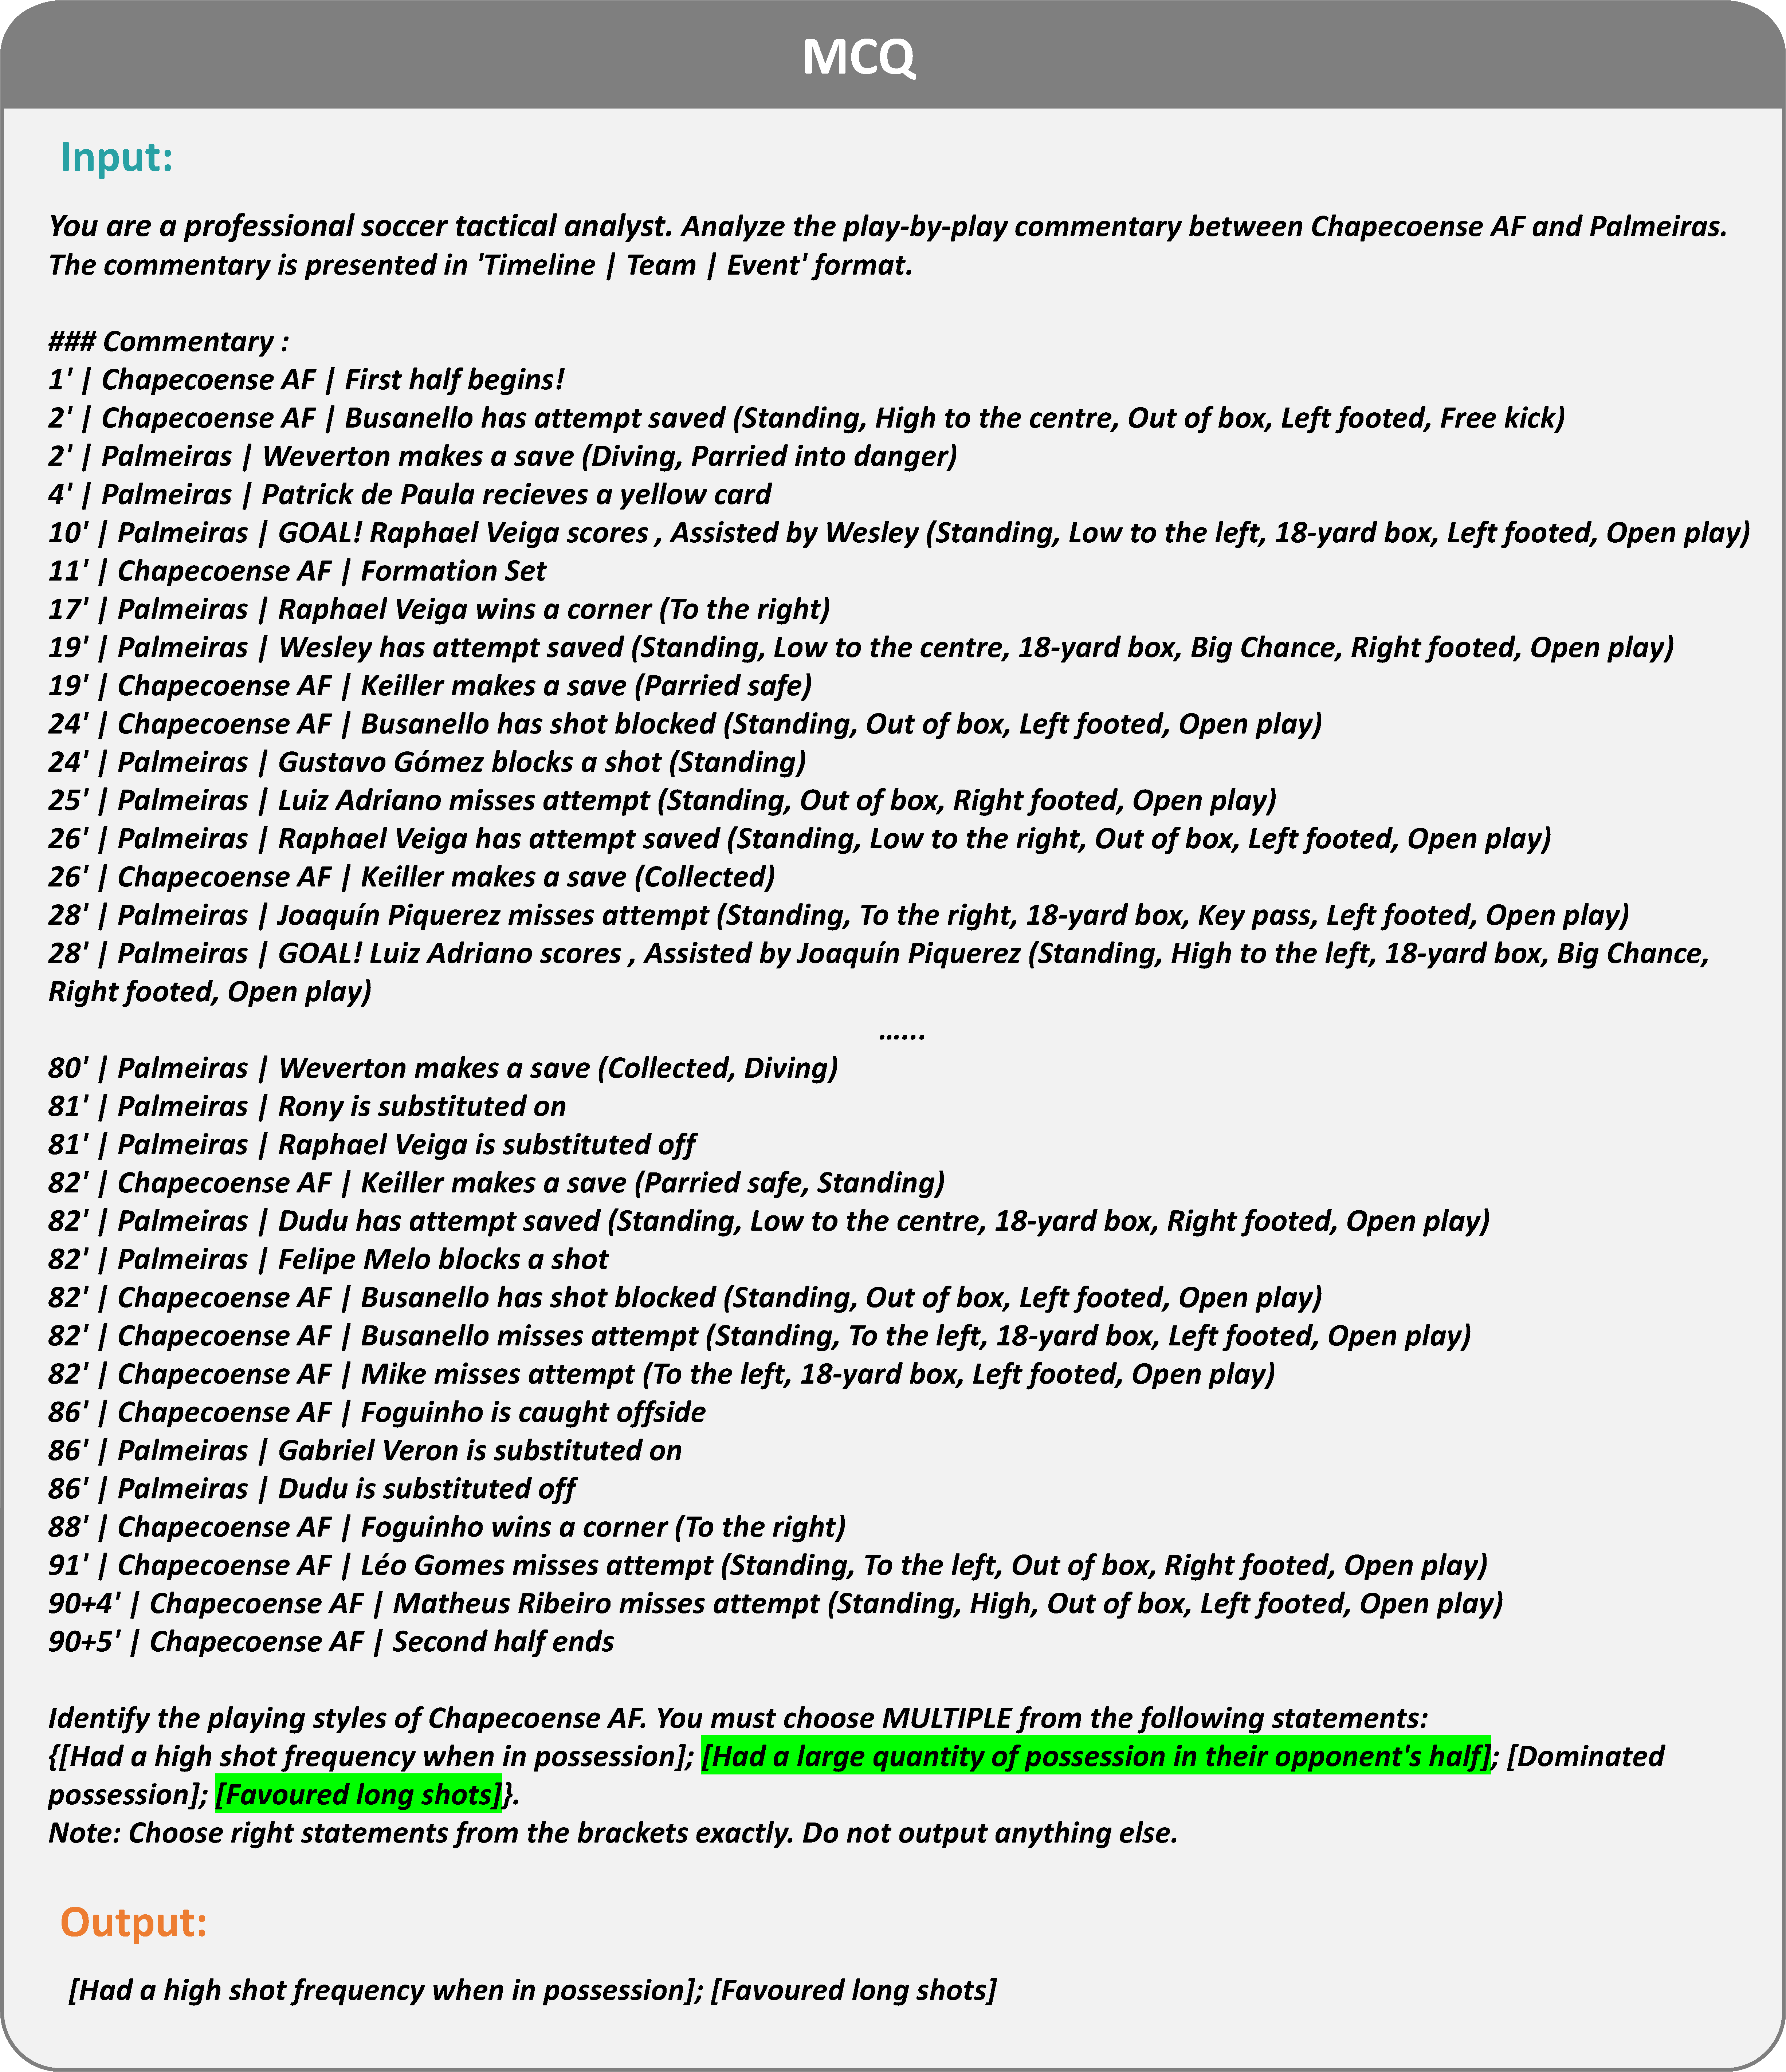
\includegraphics[width=\linewidth]{figure/figure31.pdf}
	\vspace{-5mm}
    \caption{This is a failure example of MCQ. The green sentences represent the ground truth, and the model's output does not perfectly match the ground truth. Note: Due to the length of the commentary, this example only shows a portion.}
    \vspace{-4mm}
	\label{fig:failure1}
\end{figure*}



\begin{figure*}[!t]
	\centering
	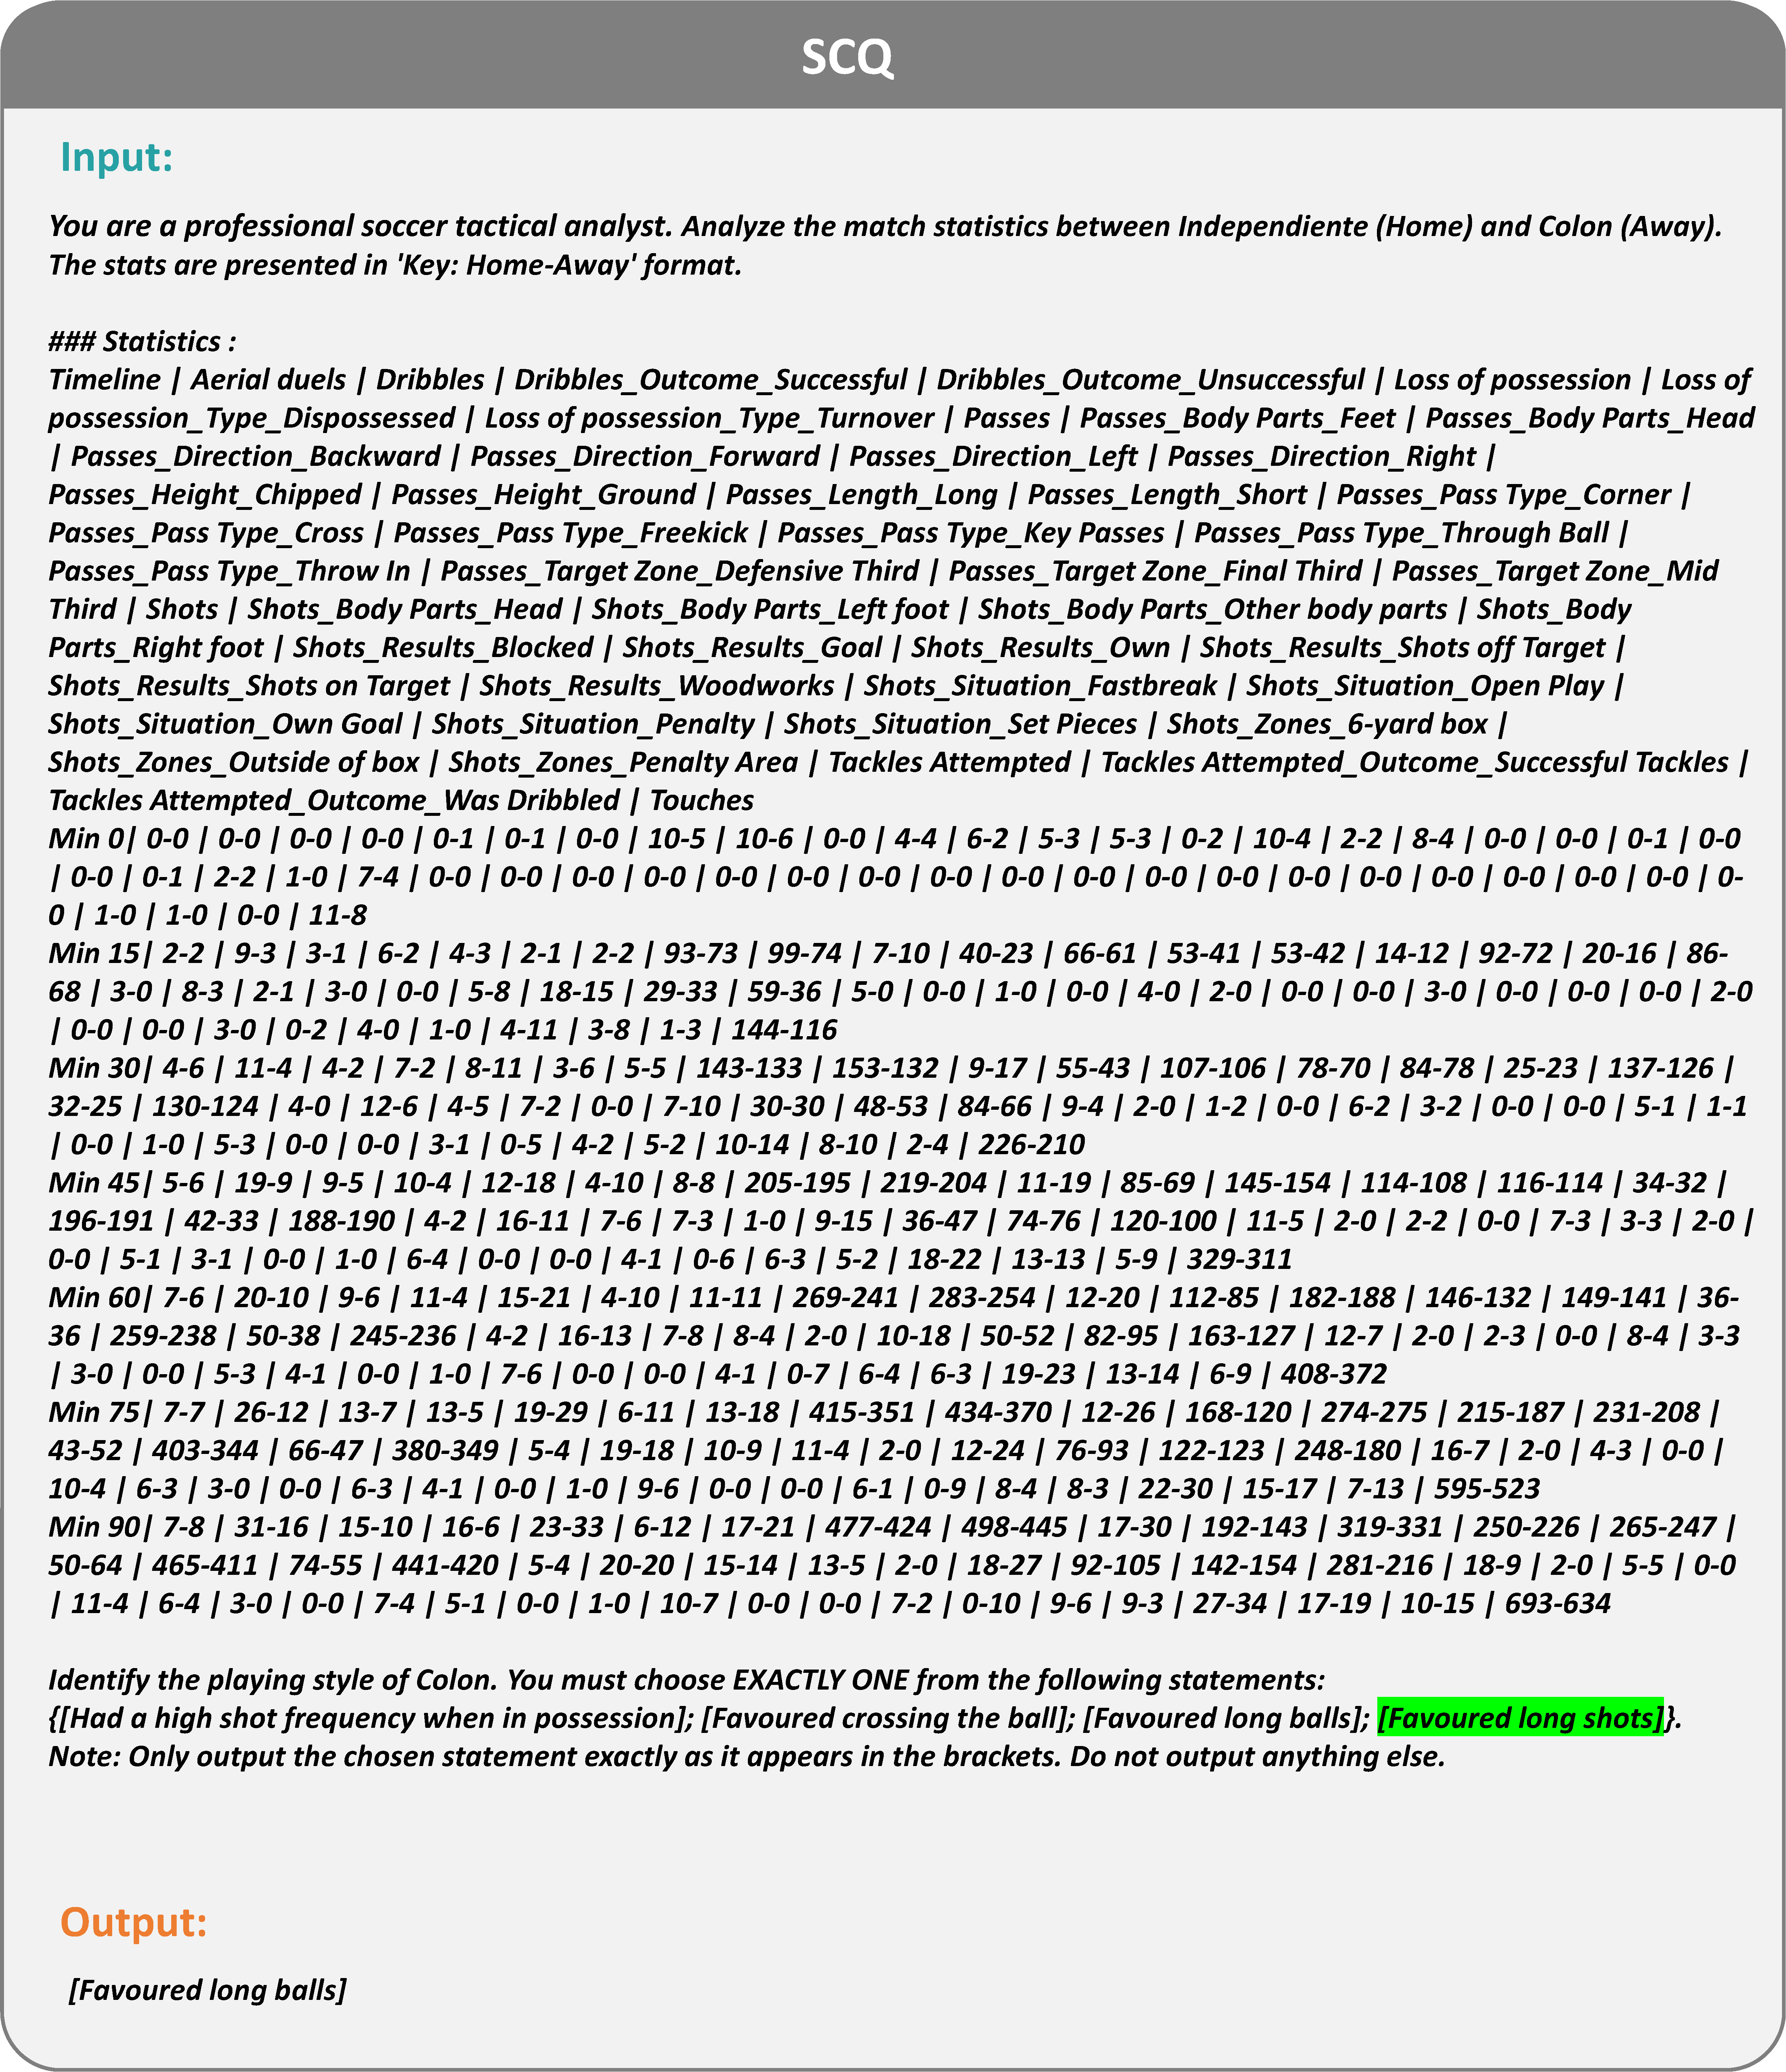
\includegraphics[width=\linewidth]{figure/figure32.pdf}
	\vspace{-5mm}
    \caption{This is a failure example of SCQ. The green sentences represent the ground truth, and the model's output does not match the ground truth.}
    \vspace{-4mm}
	\label{fig:failure2}
\end{figure*}

\begin{figure*}[!t]
	\centering
	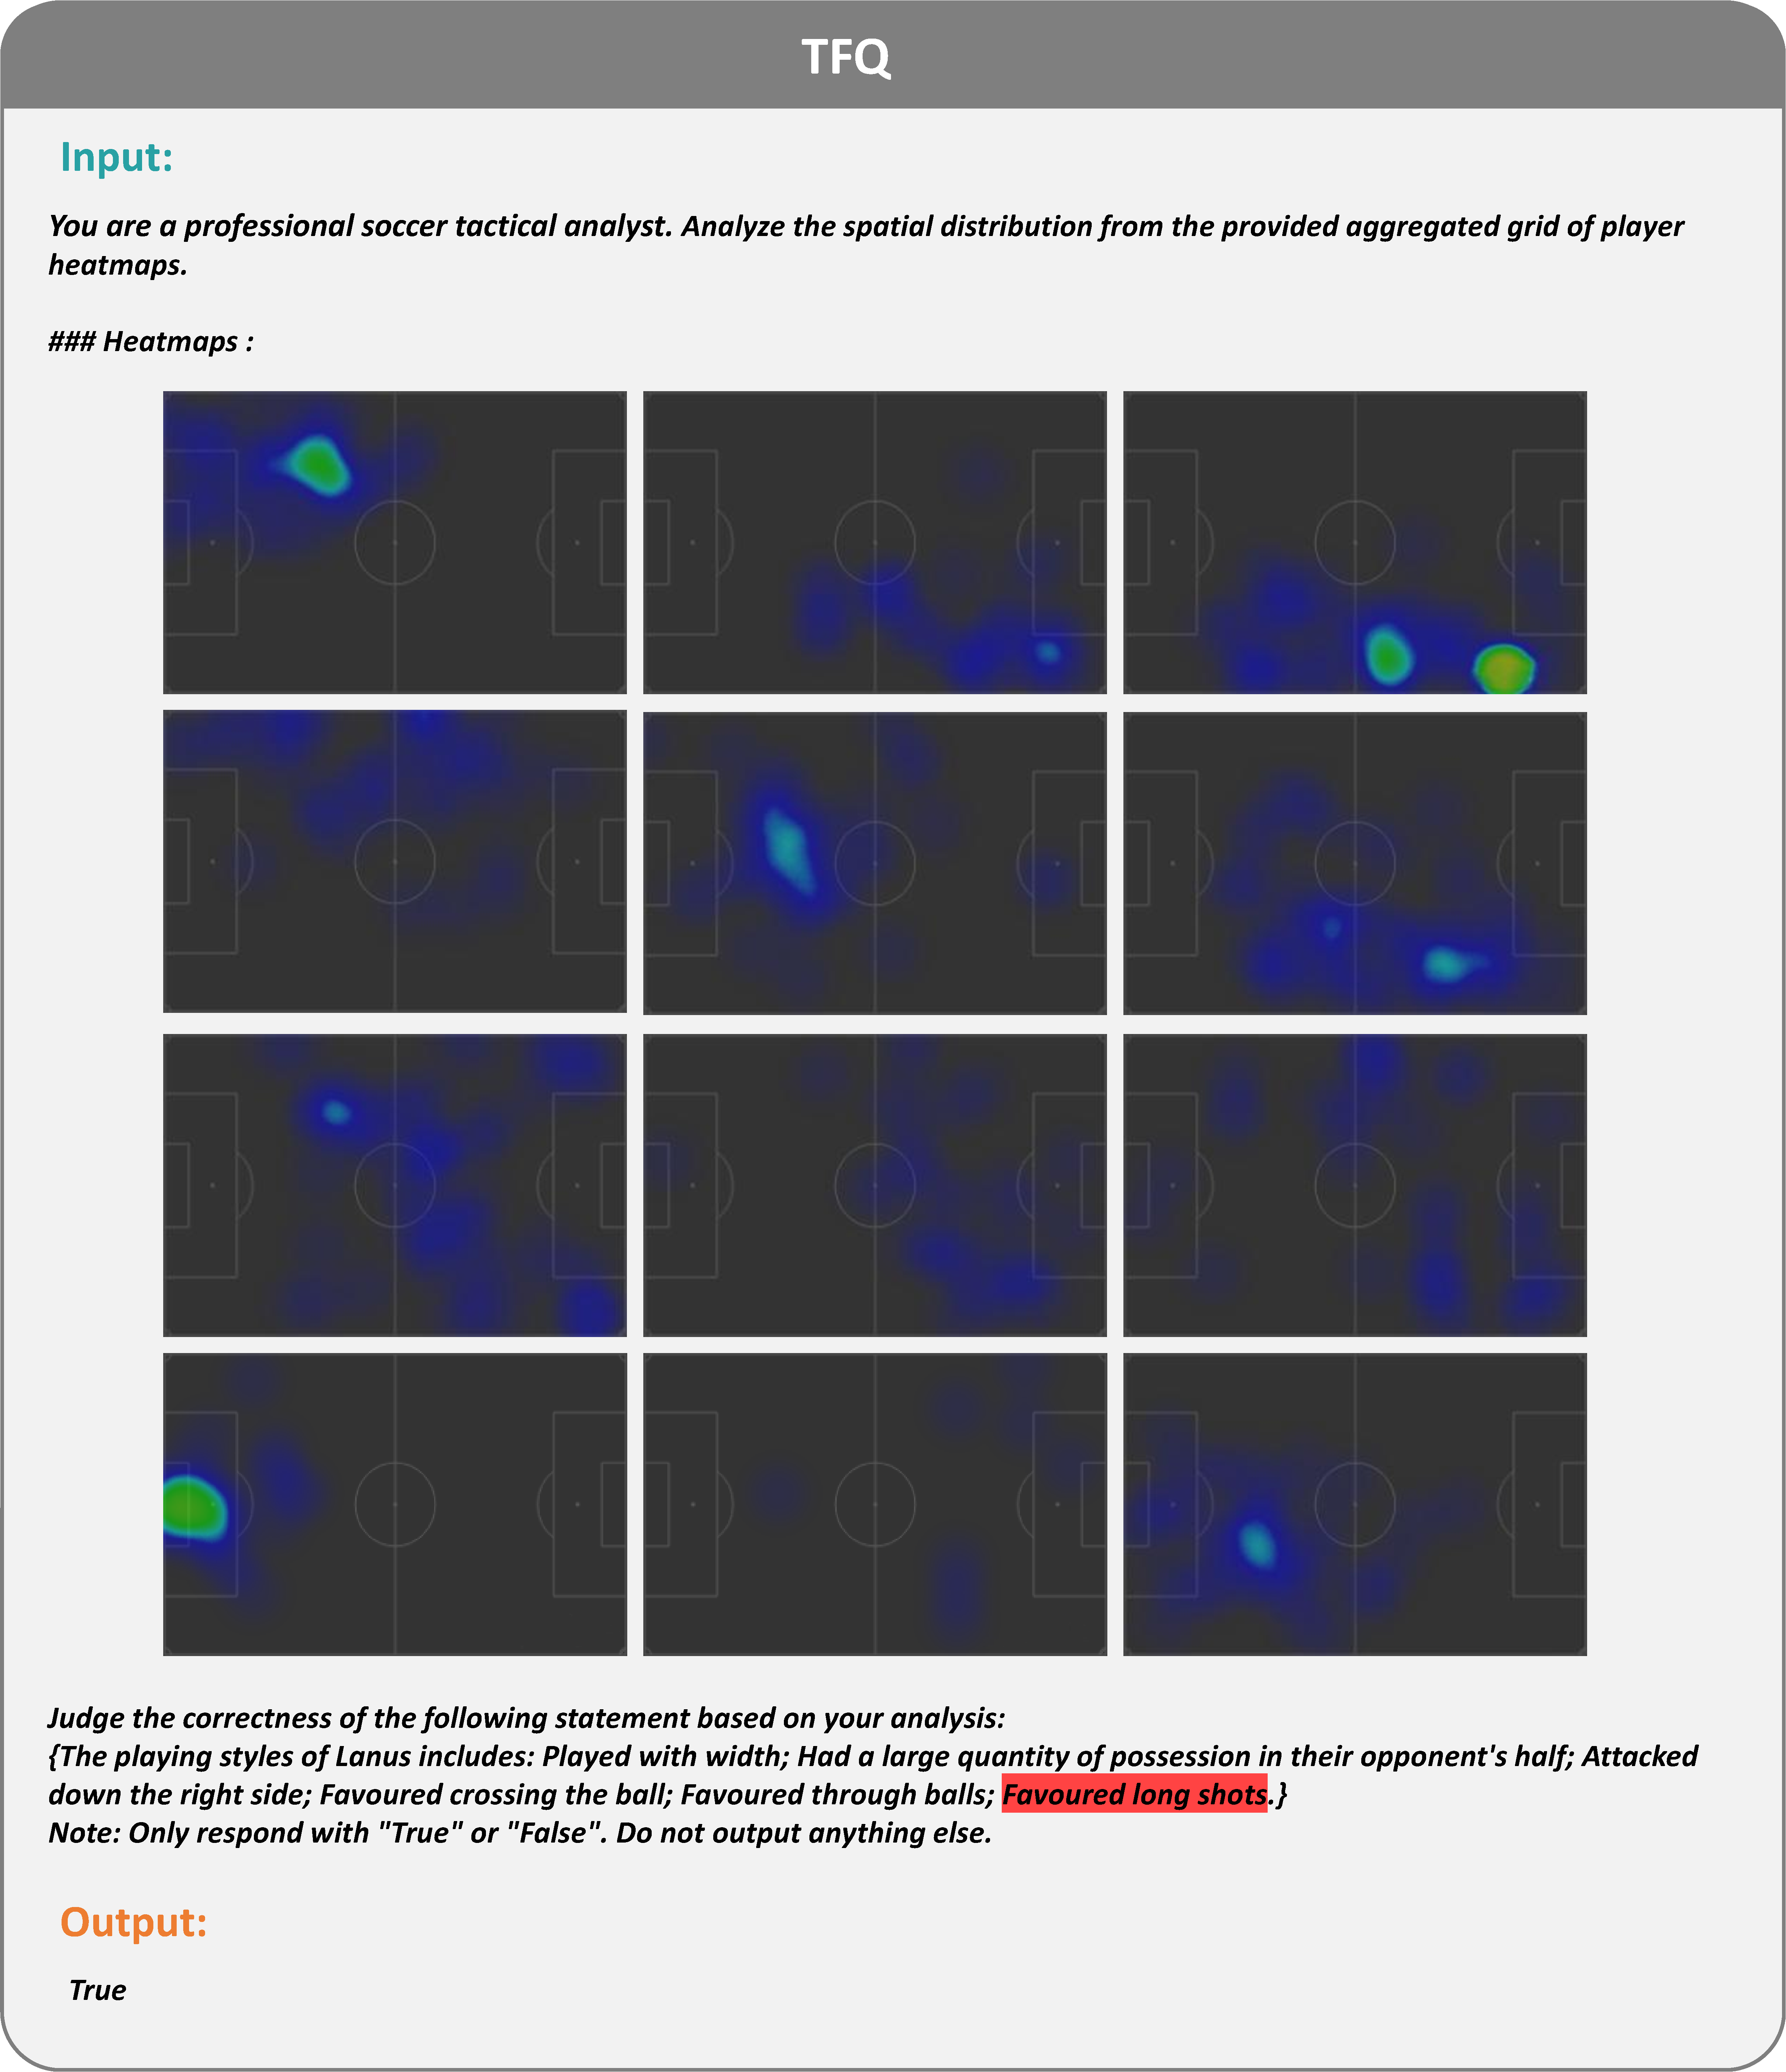
\includegraphics[width=\linewidth]{figure/figure34.pdf}
	\vspace{-5mm}
    \caption{This is a failure example of TFQ. The red sentences represent an incorrect style, but the model does not correctly identify it and considers the statement to be correct.}
    \vspace{-4mm}
	\label{fig:failure3}
\end{figure*}

\begin{figure*}[!t]
	\centering
	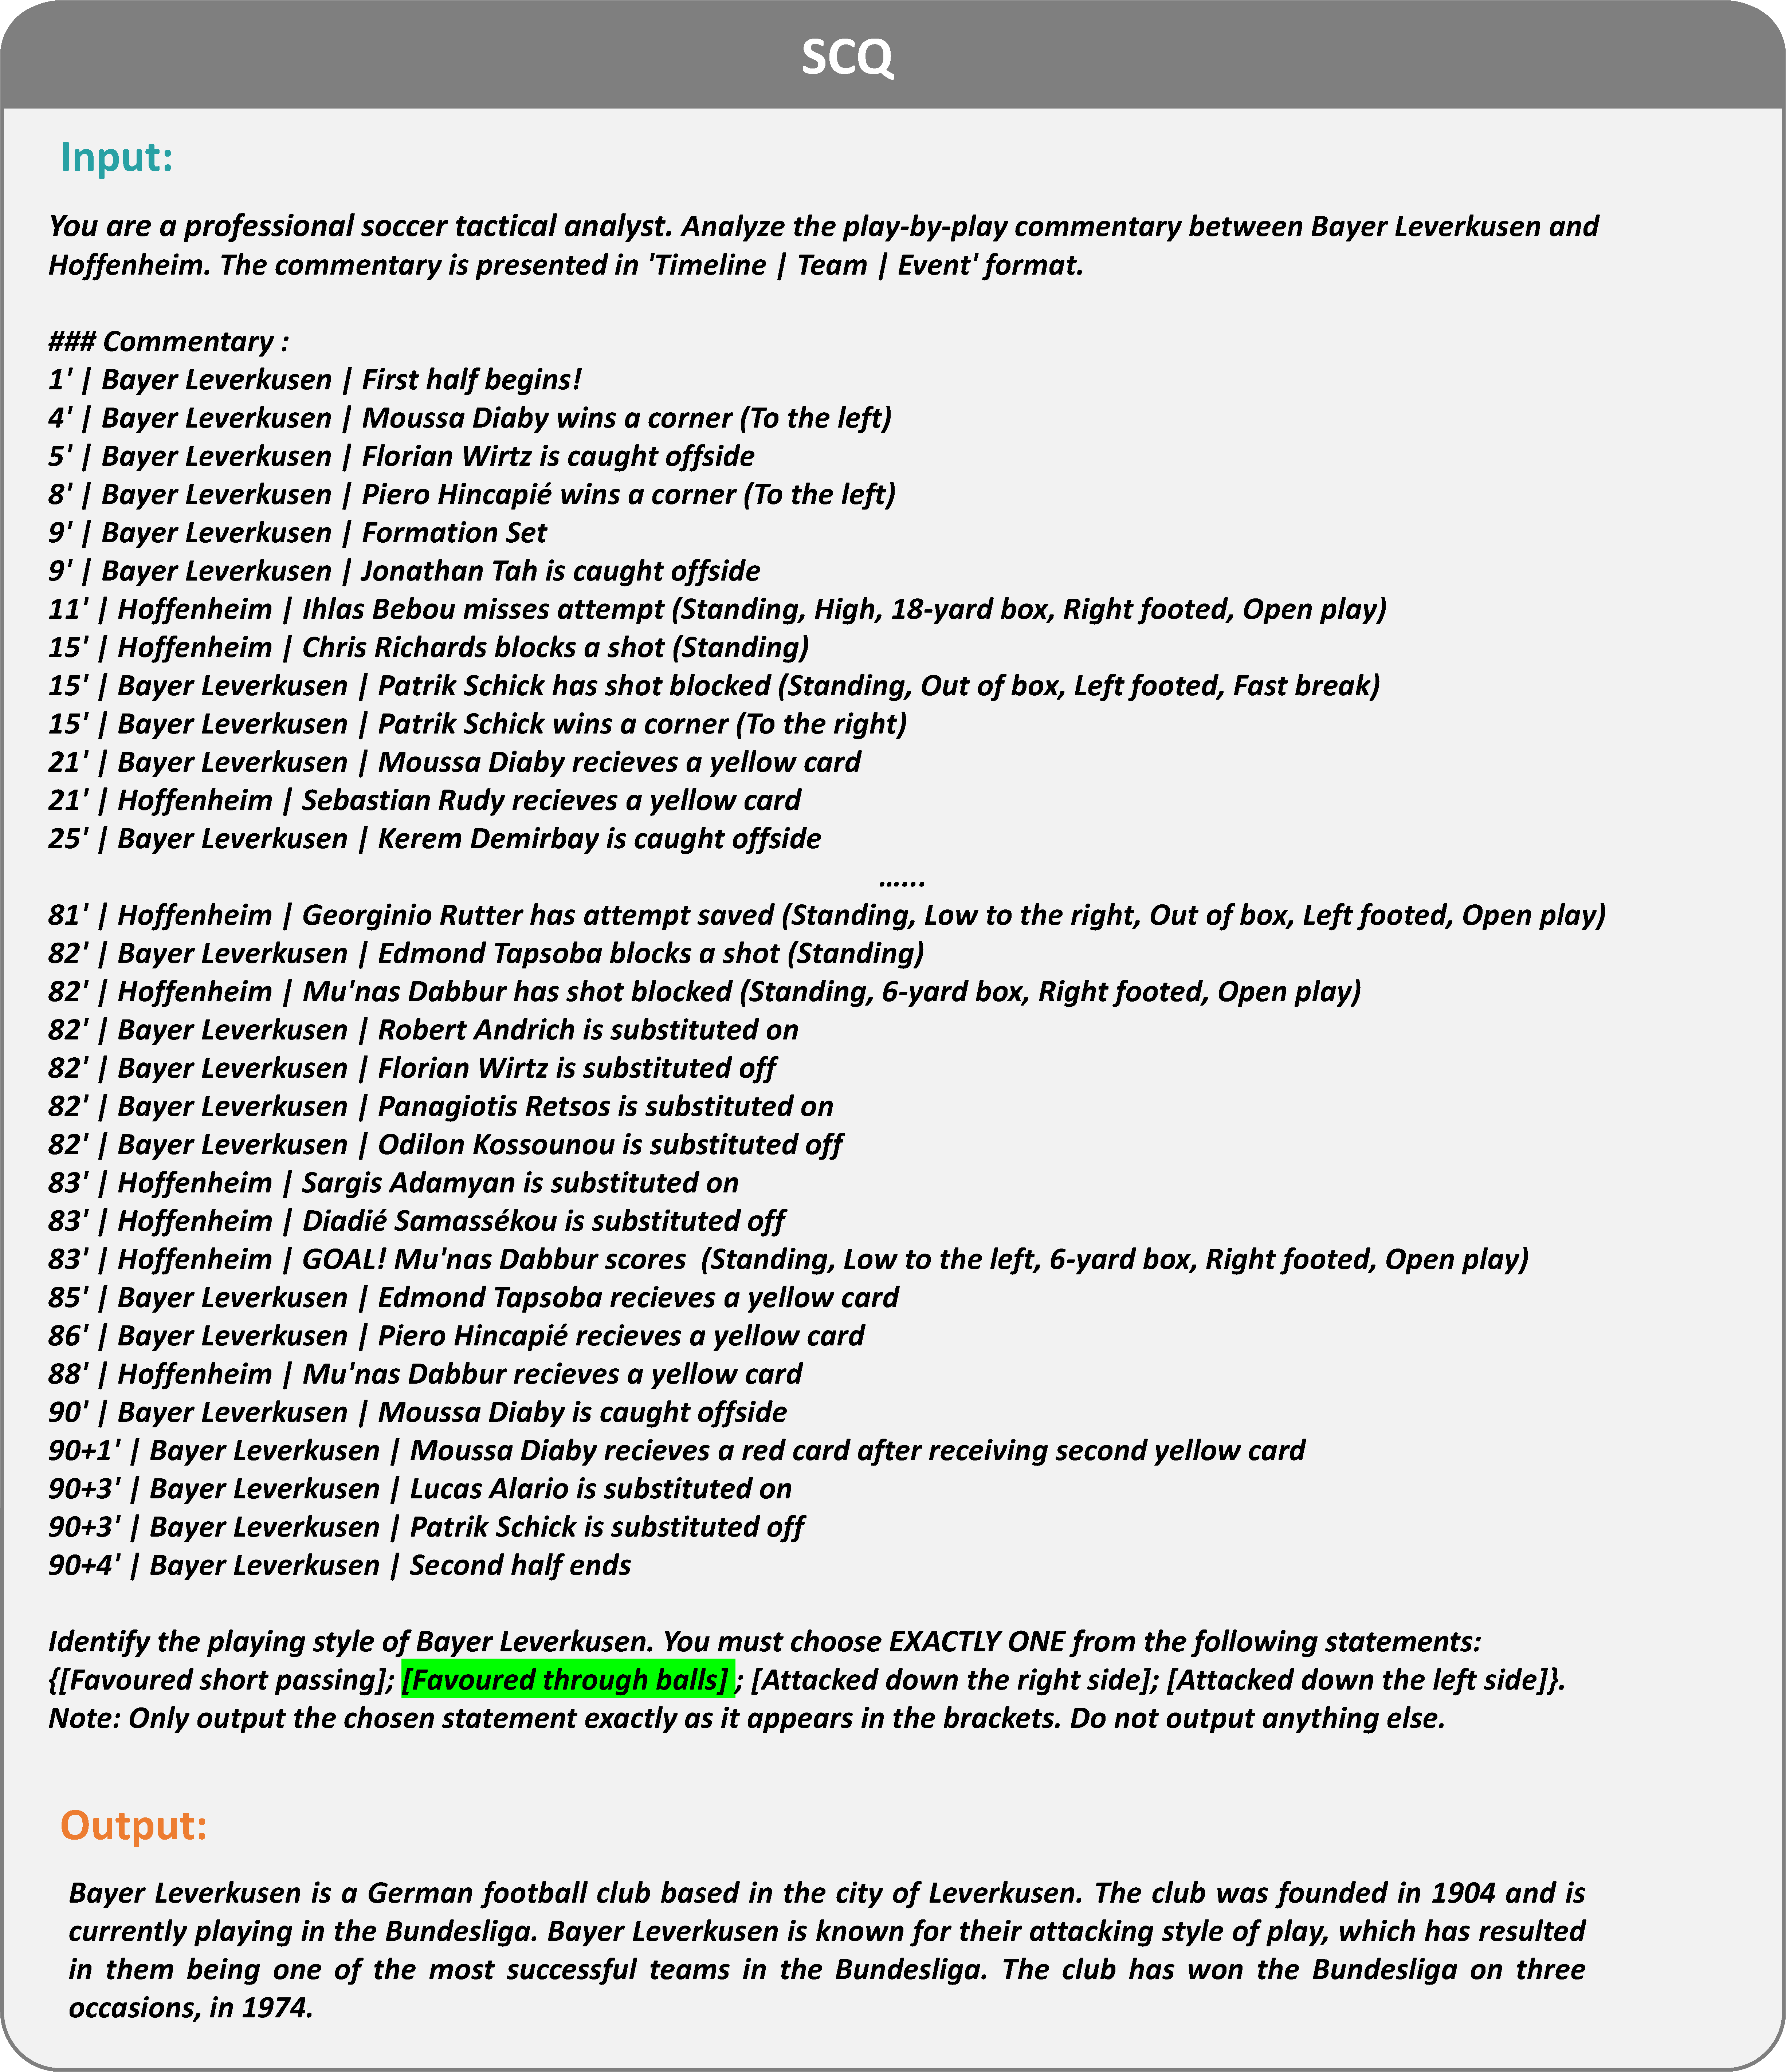
\includegraphics[width=\linewidth]{figure/figure35.pdf}
	\vspace{-5mm}
    \caption{This is a failed example with invalid output. The model is asked to perform SCQ, but its output is irrelevant text.}
    \vspace{-4mm}
	\label{fig:failure4}
\end{figure*}


%%
%% If your work has an appendix, this is the place to put it.
\appendix

\end{document}
\endinput
%%
%% End of file `sample-sigconf-authordraft.tex'.
